\documentclass[11pt, handout]{beamer} % To remove reveals for printing.
%\documentclass[12pt]{beamer}


\usepackage{color}
\usefonttheme{professionalfonts} % using non standard fonts for beamer
\usefonttheme{serif} % default family is serif
%\usepackage{fontspec}
%\setmainfont{Liberation Serif}
\definecolor{blank}{gray}{1} %1 to hide


\graphicspath{{.}{Figures/}}
\usetheme{boxes}
% 
% 
% \documentclass[handout]{beamer} % To remove reveals for printing.
% %\documentclass{beamer}
% 
% 
% \usepackage{color}
% \definecolor{blank}{gray}{0.5} %1 to hide
% 
% 
% 
% \usetheme{CambridgeUS}

\newcommand{\bx}{\mbox{$\mathbf{x}$}}
\usepackage{amsfonts}           % let's be fancy:
\def\BE{\mathbb{E}}             % E(X) -- expectation
\def\BP{\mathbb{P}}             % P(X=1) -- probability
\usepackage{graphicx}           % import and rescale EPS figures
%\usepackage{pnas}
%\usepackage{showkeys}           %shows references
\usepackage{setspace, amsthm}
\usepackage{graphicx}
\usepackage{amsbsy,amssymb,amsmath, amsthm, psfrag}



\def\pgfb[#1][#2]{\pi(#1|#2)}
\def\vv{$^\wedge$}
\def\pgfa[#1][#2][#3][#4][#5][#6]{\pi(#1_{0:#2} #3|#4_{0:#5} #6)}

\def\pgf[#1][#2][#3][#4]{\pi(#1_{0:#2} |#3_{0:#4},\theta, \psi )}
%pgf for when we have x and z on separate sizes, with phi and theta in the conditional 
\def\xt {x_{0:t}}
\def\xtp{x_{0:t+1}}
\def\zt{z_{0:t}}
\def\ztp{z_{0:t+1}}

\def\rd {\mathrm{d}}


\addtolength{\topmargin}{0cm}  % decrease the margins
\addtolength{\textheight}{0cm}
\addtolength{\oddsidemargin}{0cm}
\setlength{\evensidemargin}{\oddsidemargin}
\addtolength{\textwidth}{0cm}

\def\ignore#1{{}}
\def\stnote#1{\textbf{\large #1}\marginpar{$\spadesuit$}}
\def\no{\noindent}
\def\etal{{\it et al. }}
\def\CD{\mathcal{D}}
\def\CN{\mathcal{N}}
\def\bm#1{{{\mbox{\boldmath $#1$}}}}  
\def\Var{\mathbb{V}\mbox{ar}}
\def\rd{\rm{d}}
   \newcommand{\eps}[1]{\(\epsilon_#1 \)}
\def\bias{\mbox{bias}}
\def\htheta{\hat{\theta}}
   
  \def\se{\mbox{se}} 
\def\hF{{\hat{F}}}
 \def\BI{\mathbb{I}}
 \def\Xi{X_{i}}
 \def\xi{x_{i}}
 \usepackage{mathtools}
\newcommand\simiid{\stackrel{\mathclap{\normalfont\mbox{\tiny{iid}}}}{\sim}}

 \def\cor{\mbox{cor}}
   
\def\endexample{{\begin{flushright} $\square$ \end{flushright}}}

\setbeamertemplate{enumerate items}[default]
\setbeamertemplate{itemize items}[default]



\begin{document}

\frame{\frametitle{MAS472/6004: Computational Inference} 
\begin{center}
\Huge{ 
Chapter II\\
 Simulation methods in inference}
\end{center}
}


\frame{\frametitle{Introduction}

Classical statistical theory contains many methods for testing hypotheses in numerous different situations. 

\medskip
Derivation of these tests can be difficult or impossible in some cases and often relies on asymptotic results or approximations.  

\medskip
If the test we wish to perform is non-standard then deriving a suitable test procedure may not be possible (or we may have forgotten the correct test!).

\medskip
 In this Chapter we consider what can be done using simulation methods.
}



\frame{\frametitle{2.1 Monte Carlo tests}

\framesubtitle{Recap of hypothesis testing framework}

Suppose that we have a null hypothesis $H_0$ represented by a completely specified model and that we wish to test this hypothesis using data $X_1, \ldots, X_n$. We proceed as follows
{\color{blank}\begin{enumerate}
 \item Assume $H_0$ is true.
\item Find a test statistic $T(X_1, \ldots, X_n)$ for which large values indicate departure from $H_0$.

\item Calculate the theoretical sampling distribution of $T$ under $H_0$.

\item The observed value $T_{obs}=T(x_1, \ldots, x_n)$ of the test statistic is compared with the distribution of $T$ under $H_0$. Either
\begin{itemize}
 \item  (Neyman-Pearson) reject $H_0$ if $T_{obs}>c$. Here $c$ is chosen so that $\BP(T\geq c| H_0)=\alpha$ where $\alpha$ is the size of the test, i.e., $\BP(\mbox{reject } H_0 | H_0 \mbox{ true})=\alpha$.
\item (Fisher) compute the p-value $p=\BP(T\geq T_{obs}|H_0)$ and report it. This represents the strength of evidence against $H_0$.

\end{itemize}

\end{enumerate}
}
}

\frame{\frametitle{Example: normal parametric test}
 Suppose $X_1, \ldots, X_n \simiid N(\mu, \sigma^2)$. Suppose that   $\sigma^2=1$ is known. Consider the null hypothesis  $$H_0: \mu=0.$$

{\color{blank} Testing proceeds as follows:
\begin{enumerate}
\item {\color{blank}Assume $\mu=0$.}
\item {\color{blank}The Neyman-Pearson lemma that a suitable test statistic is $T({\bf X})=\frac{1}{n}\sum X_i$.}
\item {\color{blank}Under $H_0$ we can show $T \sim N(0, \frac{\sigma^2}{n})$ so that $Z=n^{1/2}T/\sigma \sim N(0,1)$.}
\item {\color{blank}If $Z_{obs}=2$ then we find the p-value $\BP(Z \geq Z_{obs} | H_0)=1-\Phi(2)=0.023$ and so we reject $H_0$ at the 5\% level.}
\end{enumerate}



What test do we perform if $\sigma^2$ is unknown? What about if the $X_i$ have t-distributions rather than normal distributions? What if the $X_i$ are not iid?
}
%% Note on power?
}



\frame{\frametitle{}

It may not be possible to derive the sampling distribution of $T$ under $H_0$.   
\begin{itemize}
 \item 

$T$ is not some fairly simple function, 

\item
or if $X_1, \ldots, X_n$ are not independent samples from the population of interest (dependent data are common in real problems). 


\end{itemize}

Moreover, in deriving the distribution of $T$, we assume that $n$ is large, equal variances, normality etc. If these assumptions don't hold then our distribution for $T$ will be incorrect.



}



%%%%%%%%%%%%%%%%%%%%%%%%%%%%%%%%%%% MONTE CARLO TESTS

\frame{\frametitle{Monte Carlo Tests}
We may not know the distribution of $T$ under $H_0$, but often it is possible to simulate from the model to produce sample data sets 
$$\{X_1^{(i)}, \ldots, X_n^{(i)}\}$$
 for $i=1, \ldots, m-1$. 

\medskip
From these we can calculate $m-1$ sample values of the statistic under $H_0$, $$\{T_1,\ldots, T_{m-1}\}$$ 

We can then estimate the distribution of $T$ under $H_0$ from this sample and can estimate the critical value $c$ or the p-value by a Monte Carlo approximation, i.e., estimate $\BP(T>T_{obs}|H_0)$ by 
$$\frac{1}{m-1} \sum_{i=1}^{m-1} \mathbb{I}_{T_i>t_{obs}}.$$
 }



%\frame{\frametitle{Monte Carlo Tests}
%
%To construct a test of size $\alpha$ 
%\begin{itemize}
% \item Set $k=m\alpha$ 
%\item Under $H_0$, the probability  that $t_{obs}$ is the $k^{th}$ largest or larger of the set $\{T_1, \ldots, T_{m-1}, t_{obs}\}$ is $k/m=\alpha$.
%
%\item Reject $H_0$ if $t_{obs}\geq T_{(m-k)}$ 
%
%\end{itemize}
%
%\medskip
%
%Here $T_{(1)}, \ldots, T_{(m)}$ are the order statistics of $T_1, \ldots, T_{m-1}, t_{obs}$.
%
%\medskip
%
% The reason for using $m-1$ simulated samples is that it makes a total of $m$ observations from $H_0$ when we include the observation $t_{obs}$. This makes choosing $m$ and $k$ simpler.
%
%}
\frame{
\vspace{1cm}
\fbox{
\parbox{10cm}{\begin{enumerate}
 \item[]{\bf  Monte Carlo Testing Algorithm}
 \item Generate $m-1$ sample test statistics $t_1, \ldots, t_{m-1}$ according to $H_0$.
\item Define $k=m\alpha$ (with $m$ chosen so that $k$ is an integer). If $t_{obs}$ is one of the $k^{th}$ largest values in $\{T_1, \ldots, T_{m-1}, t_{obs}\}$ then reject $H_0$.
\end{enumerate}}}

\bigskip
i.e. reject $H_0$ is $t_{obs}>T_{(m-k)}$

\medskip
where $T_{(1)}, \ldots, T_{(m)}$ are the order statistics of $T_1, \ldots, T_{m-1}, t_{obs}$.
}

\frame{\frametitle{Example: normal parametric test revisited}
 In this simple case we know the distribution of $T$ under $H_0$, but it is informative to consider the Monte Carlo test. 
 
\begin{enumerate}
 \item Generate $1000$ samples of size $n$ from a $N(0, \sigma^2)$ distribution and calculate $T$.

\qquad\texttt{t.sample <- c()\\
\qquad for(i in 1:999)\{\\
\qquad\qquad temp <- rnorm(n=n, mean=0, sd=sigma) \\
\qquad\qquad\texttt{t.sample[i] <- mean(temp)}\\
\qquad\}\\
\qquad z.sample <- t.sample*sqrt(n)/sigma\\
\qquad z <- c(z.sample, 2)  \#} recall $Z_{obs}=2$

\end{enumerate}
}

\frame{


For $\alpha=0.05$, we find the 95th percentile of the sampling distribution

\medskip
\qquad\texttt{c<-quantile(z, 0.95)}

\medskip
Then we compare $c$ with the observed value of 2. I found $c=1.67$ so we would reject $H_0$ at the 5\% level.

\medskip
If instead, we wanted to estimate the p-value $\BP(T\geq T_{obs}|H_0)$ we could estimate it using the R command

\medskip
\qquad\texttt{sum(z>2)/1000}

\medskip
For my implementation I found a p-value of 0.028 which again suggests we should reject $H_0$ at the 5\% level. 

\medskip
Note that this is a random test:  if we repeat it multiple times we will get a slightly different answer each time.


}



\frame{\frametitle{Example: Chi-squared tests} %% Set as a class example.
Exam grades are to be compared between 16 boys and 19 girls in a single class. The data are
\begin{center}
\begin{tabular}{|c|cccc|}
\hline
&A&B&C&D\\
\hline
boys&3&4&5&4\\
girls & 8&8&3&0\\
\hline 
\end{tabular}
\end{center}

\medskip
The null hypothesis is that there is no difference between boys and girls in exam performance.

\medskip
In other words,
a girl and boy chosen at random have the same probability of obtaining any particular grade. 

}

\frame{
To apply the standard chi-squared test in this case we would calculate the table of expected values under $H_0$ and then calculate the test statistics 
{\color{blank}
\begin{equation}\label{eqn:chi2}
T=\sum\frac{(O_i-E_i)^2}{E_i}
\end{equation}}

Calculating for the data we find $T_{obs}=7.907$, which has a p-value of 0.048.


\medskip
However, as a rule of thumb, to use the $\chi^2$ test, the expected number of counts in each cell should be at least 5. In this case,  4 of the 8 values are less than 5, which means the assumptions used to show that $T$ has a $\chi^2$ distribution with 3 degrees of freedom do not hold. %To get round this we could merge cells (although we get the same results).

}

\frame{
Consider using a Monte Carlo test to perform the test. 
\begin{enumerate}
 \item Under $H_0$, probabilities of obtaining each grade are given by the estimates
\begin{center}
\begin{tabular}{|c|cccc|}
\hline
&A&B&C&D\\
\hline
probability & $\frac{11}{35}$& $\frac{12}{35}$  &  $\frac{8}{35}$  & $\frac{4}{35}$\\
\hline 
\end{tabular}
\end{center}

\item We then generate a new set of results for boys and girls; the boys' results are sampled from a Multinomial$(16, \frac{11}{35}, \frac{12}{35},   \frac{8}{35}, \frac{4}{35})$ distribution, and the girls' from a  Multinomial$(19, \frac{11}{35}, \frac{12}{35},   \frac{8}{35}, \frac{4}{35})$. An example is shown below:

\begin{center}
\begin{tabular}{|c|cccc|}
\hline
&A&B&C&D\\
\hline
boys&3&5&6&2\\
girls & 4&5&7&3\\
\hline 
\end{tabular}
\end{center}

\item Calculate  $T$ for these data, which for this simulated dataset is 5.323.

\end{enumerate}
We then repeat $m-1$ times to get $T_1, \ldots, T_{m-1}$
}



\frame{
We rank $T_1, \ldots, T_{m-1}$ together with the observed value of the test statistic $T_{obs}$. In R we generate 99 test statistics and find 75 to be less than $T_{obs}$, and 24 to be greater. In this case the null hypothesis is not rejected at the 5\% level. 

\medskip
Notice that this is a different conclusion to that reached using the $\chi^2$ test.

\medskip

{\bf In this case, the Monte Carlo test should preferred as we are working with the true distribution of the test statistic and not an approximation. }

\medskip
In general, when conducting hypothesis tests we do not have to be so reliant on distributional approximations, and {\bf we should always consider the option of working with exact distributions}.
}


\frame{\frametitle{Example 2: Testing for randomness in
spatial patterns}\pause $H_0$: The spatial locations of each subject
are randomly distributed over the unit square: both coordinates have
$U[0,1]$ distributions. \pause $$$$  Various possibilities for test
statistic. We will consider \textit{nearest-neighbour} of each
subject.\pause $$ $$ Let $d_i$ denote distance from subject $i$ to
next closest subject, and define the test statistic $T$ to be
\begin{equation}
T=\left(\sum_{i=1}^{50}d_i\right)^{-1}.
\end{equation}\pause
If locations are clustered, nearest neighbours will be small
$\Rightarrow T$ will be large. }

\frame{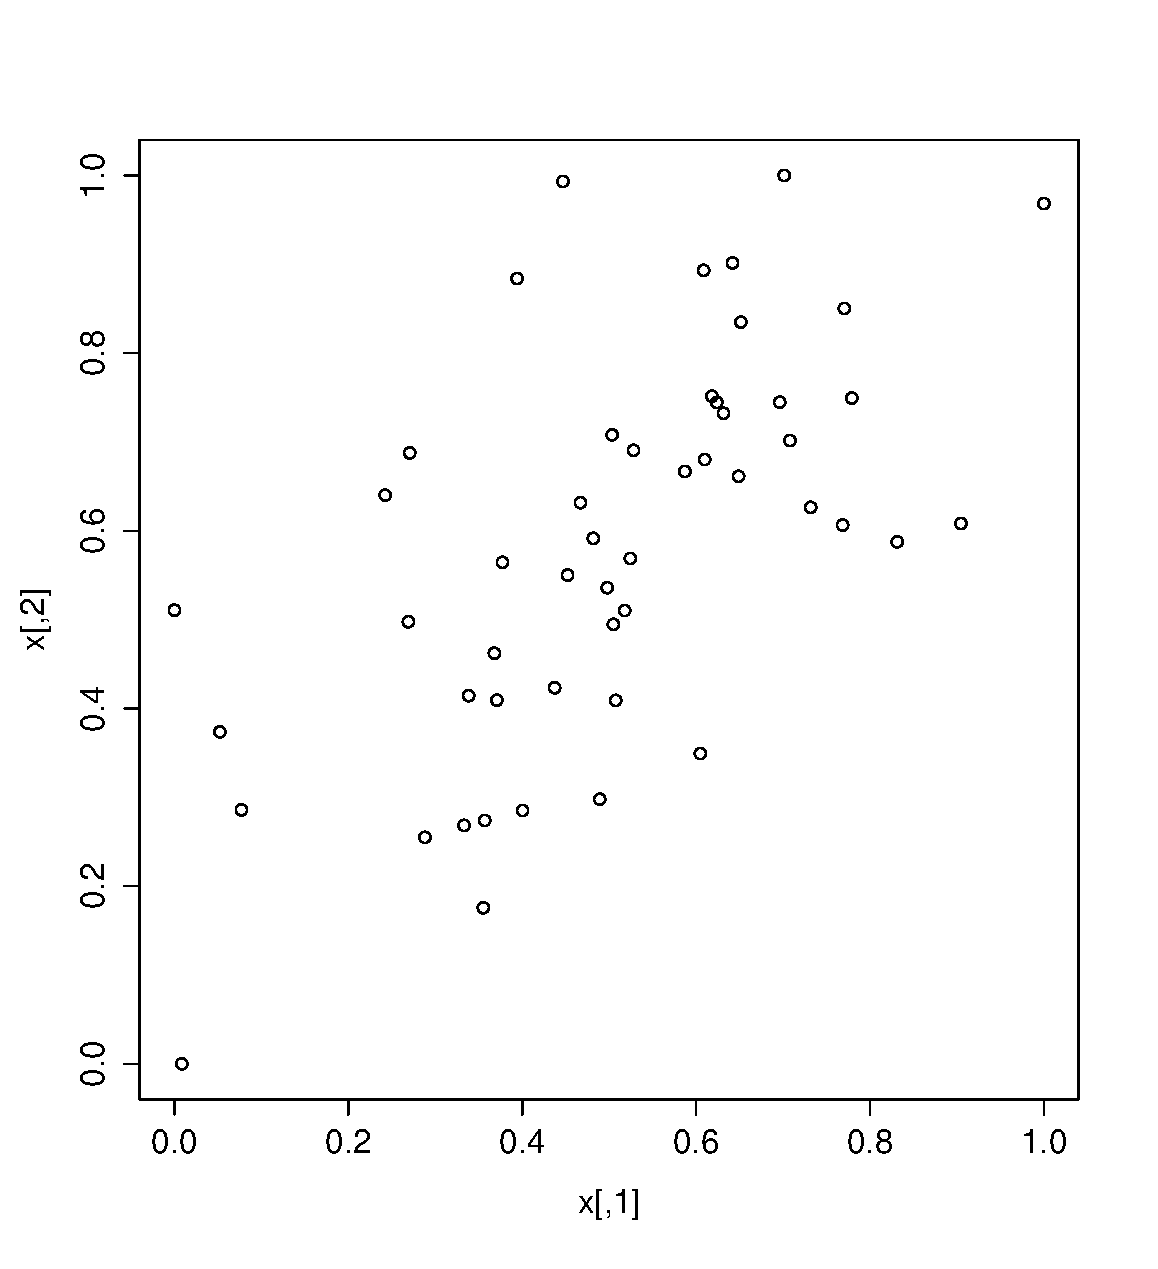
\includegraphics[width=0.7\textwidth]{clustered.eps}}


\frame{

 Under $H_0$, don't know theoretical
sampling distribution of $T$. Straightforward to simulate values of
$T$ under $H_0$, so can estimate the critical values (such as the
95th percentile) we need for the hypothesis test.\pause
\begin{enumerate}
\item Generate locations $(x,y)$ of each subject by sampling $x$
and $y$ independently from $U[0,1]$.\pause
\item For each subject, find the closest observation and measure
the distance to it to obtain the nearest-neighbour distance for that
observation\pause \item Take the reciprocal of the sum of the 50
nearest-neighbour distances to get $T_i$.
\end{enumerate}\pause

Given a sample $T_1,\ldots,T_{m-1}$, we then rank
$T_1,\ldots,T_{m-1}$ and the observed $T_{obs}$ in order to give
$T_{(1)},\ldots,T_{(m)}$. For a test of size $5\%$, if $T_{obs}$ is
one of the $0.05\times m$ largest values, then $H_0$ is rejected. }




% another example - points from JEO or dependent sample etc?
\frame{\frametitle{p-values}
We can estimate the p-value $\BP(T\geq T_{obs}|H_0)$ of a Monte Carlo test by looking at the number of observations greater than $T_{obs}$

$$\hat{p}=\frac{1}{m}\left(\sum_{i=1}^{m-1} \mathbb{I}_{T_i \geq T_{obs}}+1\right)$$

{\bf Exercise: } If $p=\BP(T\geq T_{obs}|H_0)$ show that $$\sum_{i=1}^{m-1} \mathbb{I}_{T_i \geq T_{obs}} \sim Bin(m-1, p)$$ so that the estimate $\hat{p}$ has expectation
$$\BE(\hat{p})=p+\frac{1-p}{m}$$
and is therefore a biased estimator of $p$. Note that for large $m$ the bias is small.

}



\frame{\frametitle{How large should $m$ be?}

We need to choose $m$ sufficiently large so that the random sample $T_1, \ldots, T_{m-1}$ allows us to estimate the critical region to a sufficient degree of accuracy.


\medskip
The Monte Carlo test has a random critical point and so `blurs' the critical region. 

\begin{itemize}
 \item 
We reject $H_0$ if $T_{obs}$ is one of the $k-1$ largest values in $\{T_1, \ldots, T_{m-1}\}$, where $m=k \alpha$.

\item
If $p$ is the true p-value then we reject $H_0$ with probability
\begin{align*}
R(p)&=\sum_{r=0}^{k-1}{m-1 \choose r}p^r(1-p)^{m-r-1}\\
&= \BP(\operatorname{Bin}(m-1,p) \leq k-1)
\end{align*}
\end{itemize}
}


\frame{
 \begin{center}
  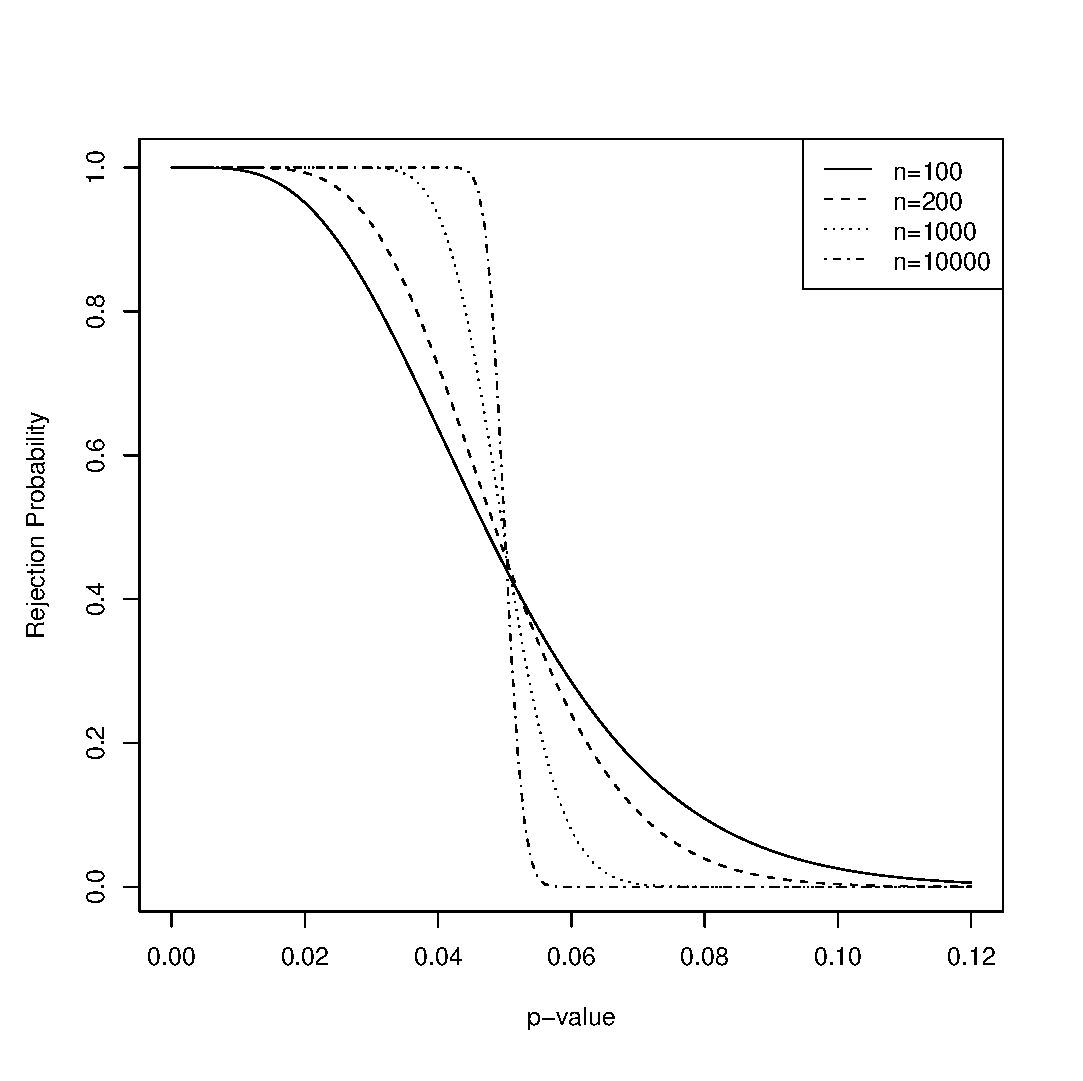
\includegraphics[scale=0.5]{MCtestRp.eps}
 \end{center}

}

\frame{
$R(p)$ can be interpreted as the proportion of times the Monte Carlo test will reject $H_0$ when we observe $T_{obs}$. 

\medskip
For p-values smaller than 0.05 we want $R(p)$ to be large and for p-values greater than 0.05 we want $R(p)$ to be small. We choose $m$ to make this so.


\medskip
We conclude from the figure that a sample size of $m=99$ is usually acceptable as long as the results aren't interpretted too rigidly. 




\medskip
Of course, this is only an issue if generating test statistics requires substantial computational effort. If it is trivial to generate sample test statistics (which it is in all but the most complex of cases), then a much large value of $m$ can be used.

}
%%%%%%%%%%%%%%%%%%%%%%%%%%%%%%%%%%%%%%%%%%%%%%%%%%%%%%%%%%%
%%%%%%%%%%%%%%%%%%%%%%%%%%%%%%%%%%%%%%%%%%%%%%%%%%%%%%%%%%%
%
% Randomisation tests
%
%%%%%%%%%%%%%%%%%%%%%%%%%%%%%%%%%%%%%%%%%%%%%%%%%%%%%%%%%%%
%%%%%%%%%%%%%%%%%%%%%%%%%%%%%%%%%%%%%%%%%%%%%%%%%%%%%%%%%%%




\frame{\frametitle{2.2 Randomization Tests}

We now consider a second technique for deriving the sampling distribution of the test statistic, where  no distributional assumptions about the data are required. 

\medskip
The general scenario under consideration is that of an investigation into whether or not a particular treatment/covariate/factor has an effect on some response.

\medskip

 We will illustrate the concept of the randomisation test with an example.
}






\frame{\frametitle{Example: Cholesterol data}

A small study was conducted to investigate the effect of diet on cholesterol levels. Volunteers were randomly allocated to one of two diets, and cholesterol levels were recorded at the end of the trial period

\begin{center}
\begin{tabular}{c|cccccccc}
 Diet A& 233&291&312&250&246&197&268&224\\
\hline
Diet B & 185&263&246&224&212&188&250&148\\ 
\end{tabular}
\end{center}

The interest is in whether or not there is a significant difference between the mean cholesterol levels for the two groups. The null hypothesis is

\begin{center}
 $H_0:$ mean cholesterol levels with the diets are equal
\end{center}
}

\frame{
A standard analysis of this data might be to assume $$X^{(j)}_i \sim N(\mu_j, \sigma^2)$$ for $i=1, \ldots, 8$ and $j=1,2$ with $\sigma^2$ an unknown common variance. 

\medskip
The standard test is then a two sample t-test, based on the statistic 
$$T=\frac{\bar{X}^{(1)}-\bar{X}^{(2)}}{\sqrt{s^2/8+s^2/8}},$$
where $s^2$ is the pooled estimate of variance. 

\medskip
Then under $H_0$ (and assuming normality of the data!), the test statistic $T$ has a t-distribution with 14 degrees of freedom. 

\medskip
For this data, the observed test statistic $T_{obs}$ is 2.0034 with a p-value of 0.0649 for a two-sided test. 
}

\frame{

But what if we want to analyse the data without assuming normality? 

\begin{itemize}\item Because the sample sizes are small, assuming normality may not be wise. 
\end{itemize}

\medskip
Randomization tests can be used to find a distribution for $T$ without making any distributional assumptions about the data.

\medskip
If $H_0$ is true, then any difference in the two sample means would be solely due to how the 16 individuals were assigned to the two groups. So if $H_0$ is true, what is the probability of observing a sizeable difference between the two group means? 

\medskip
It must be equal to the probability of assigning the indivuals to the two groups in such a way that the imbalance occurs, as long as the individuals were assigned to the two groups at random in the actual study. This is the principle idea behind randomisation tests. 

}


\frame{


\fbox{
\parbox{11cm}{\begin{enumerate}
 \item[]{\bf  Randomisation Test}
\item Suppose the 16 individuals in the study have been labelled
\begin{center}
\begin{tabular}{c|cccccccc}
 Diet A& 1&2&3&4&5&6&7&8\\
\hline
Diet B & 9&10&11&12&13&14&15&16\\ 
\end{tabular}
\end{center}
\item Randomly re-assign the 16 individuals to the two groups.

\item Re-calculate the test-statistic for this permuted data
\item Repeate 2 and 3 to obtain $B$ sampled test-statistics, denoted $T_1, \ldots, T_B$.

\item For a two-sided test, the estimated p-value of the observed test statistic $T_{obs}$ is
$$\frac{1}{B}\sum_{i=1}^B \mathbb{I}_{|T_i|\geq |T_{obs}|}$$


\end{enumerate}}}
Using 10000 random permutations gave a p-value of 0.063. 

\vspace{1cm}
}


\frame{\frametitle{Equivalent test statistics} \pause Significance
level of $T_{obs}$ determined using $\frac{1}{N}\sum_{i=1}^N
I\{|T_i|\ge |T_{obs}|\}$. \pause

\medskip
Notice that multiplying $T_{obs}$ and all
$T_i$s by some constant
would have no effect on significance level;
ordering would be preserved. \pause

\begin{block}{Equivalent test statistic}
Any alternative test statistic that preserves ordering and hence the
$p$-value.\end{block}
\pause
In the example, an equivalent test statistic would be
 \begin{equation}
T=\bar{X}_1-\bar{X}_2.
\end{equation}

}
% 
% \frame{\frametitle{ Why use randomisation tests?} \pause
% 
% \begin{itemize}
% 
% \item
% Samples rarely `truly' random. \pause \item No theory to generalize results
% to population \pause\item `non-statistical' judgments needed for both
% randomisation and conventional tests. \pause \item Can be used for any test
% statistic. \pause \item Doesn't assume distribution for data.
% \pause\item Can help validate conventional tests.
% 
% \end{itemize}
% 
% \pause
% Requirement is that either random allocation was explicit part of
% experimental design, or actual allocation was equally likely as
% any other.
% 
% }

\frame{\frametitle{ Exact randomisation tests} \pause

Could consider systematically \textit{every} possible permutation,
rather than a random sample of permutations to determine the
significance level. \pause

\begin{itemize}

\item  This is known as an
\textbf{exact} randomisation test or \textbf{permutation} test \pause
\item Can be computationally demanding/impracticable if number of
possible permutations is large. \pause \item A large sample of random
permutations should be sufficient.
\end{itemize}

}


  

\frame{\frametitle{Outliers}

In parametric tests, outlying observations in the data can cause problems. 
\begin{itemize}
 \item In the comparison of means problem, an outlier can increase the difference $\bar{X}^{(1)}-\bar{X}^{(2)}$ and will  inflate the within group variance.

\item Consequently the true significance of the test statistic may be underestimated.
\end{itemize}
In a randomisation test, you are comparing the relative size of the observed test statistic to its value under alternative random permutations.

\medskip
Hence, the outlier will not have the same effect. 

}

\frame{




This is illustrated in some data from a study reported in Ezinga (1976) for two treatments $A$ and $B$:
\begin{center}
\begin{tabular} {c|cccccccccc}
A& 0.33&0.27&0.44&0.28&0.45&0.55&0.44&0.76&0.59&0.01\\
\hline
B &0.28&0.80&3.72&1.16&1.00&0.63&1.14&0.33&0.26&0.63\\
\end{tabular} 
\end{center}
The sample group means are $\bar{X}_A=0.412$ and $\bar{X}_B=0.995$, and the observed test statistic for a two sample t-test is $T=1.78$. For a two-tailed test this gives a p-value of 0.11, so not significant at the 5\% level. Using a randomisation test, $T$ is now significant at the 5\% level with a p-value of about 0.03.
}
% 
% \frame{\frametitle{Exact/Permutation tests}
% In principle, it is possible to calculate the value of the test statistic for every possible permutation of the data. 
% 
% \medskip
% Computationally, it is usually simpler to estimate the significance level based on a sample of random permutations. If the sample of random permutations is large, then the estimate should be sufficiently accurate. 
% 
% \medskip
% Randomisation tests in which all permutations are evaluated are known as {\it exact tests} or {\it permutation tests}.
% }
% 

\frame{\frametitle{Example: Analysis of Variance}

Randomisation tests are applicable in many different contexts. Analysis of variance is another example. Below are responses measured on four treatment groups:

\begin{center}
 \begin{tabular}{c|ccccc}
Group A&-0.10&-1.10&0.74&-3.80\\
Group B&0.94&-0.30&0.67&0.86&1.19\\
Group C& -0.25&0.84&0.04&0.25\\
Group D&0.99&0.08&0.98&0.75&0.53\\
 \end{tabular}
\end{center}

Test the null hypothesis
\begin{center}
$H_0:$ all four groups have equal means 
\end{center}
{\color{blank}A conventional $F$  test (one-way anova) could be used: the ratio of the between-group sum of squares to the within-group sum of squares is compared with the $F_{3, 14}$ distribution. The p-value for the observed $F$ statistic is 0.08.
}}


\frame{
Alternatively, a randomisation test could be applied:
\begin{enumerate}
 \item Randomly re-assign the observations to the four treatments, keeping the numbers in each treatment the same.

\item Evaluate the test statistic
$$F=\frac{ (\sum_{i=1}^4 n_i (\bar{x}_i-\bar{x})^2)/3}{(\sum_{i=1}^{4} \sum_{j=1}^{n_i} (x_{i,j}-\bar{x}_i)^2)/14}$$
for the permuated data.
\item Repeat steps 1 and 2 $B$ times to obtain sampled test statistics $F_1, \ldots, F_B$.

\item Estimate the significance level of $F_{obs}$ by
$$\frac{1}{B}\sum_{i=1}^B \mathbb{I}_{F_i\geq F_{obs}}.$$
\end{enumerate}
Based on a sample size $B=10000$, the estimate p-value for $F_{obs}$ was 0.03, suggesting slightly stronger evidence against the null hypothesis (compared with the parametric test).
}

%add confidence intervals?


\frame{
\frametitle{One-sample randomisation tests}

Randomisation tests can be used for one-sample problems, but under stricter assumptions. This is demonstrated with the following example:


\medskip
Given observations $$\{10.61, 9.46, 7.02, 11.68, 9.58, 11.96, 11.28, 7.63, 6.42, 8.85\}$$ drawn from some population with mean $\mu$, test the null hypothesis

$$H_0: \mu=10.$$

It is not immediately obvious what can be permuted here. However, supposing the two following assumptions hold:
\begin{itemize}
 \item Each observation has been sampled randomly from its population
\item The population distribution is symmetric about its mean.
\end{itemize}
}



\frame{
Now suppose $H_0$ is true, and consider randomly sampling a value $X$ from the population, and then evalutating $Y=X-10$. If the population distribution is symmetric about 10, then $Y$ must have an equal probability of being positive or negative.

\medskip
In this example, subtracting 10 from each observation and taking the resulting mean gives a sample mean of -0.551. We will use the absolute value of this sample mean as the test statistic, so $T_{obs}=0.551$ (for a two-sided test).

\medskip
 If $H_0$ is true, and both assumptions hold, then the observed sample mean could simply be due to an imbalance of positive and negative $Y$ values. This can be tested as follows:

}

\frame{
\fbox{
\parbox{11cm}{\begin{enumerate}
%\itemsep[0em]
\item[]{\bf  Fisher's Randomisation test}
\item Subtract hypothesised population mean from each observations:
$$\!\!\!\!\!\!\{0.61, -0.54, -2.98, 1.68, -0.42, 1.96, 1.28, -2.37, -3.58, -1.15\}$$ 

\item Calculate the observed test statistics: $T_{obs}=0.551$
\item With probability 0.5 for each observation, change the sign of $X-\mu$. E.g.
$$\!\!\!\!\!\!\!\!\!\!\{-0.61, -0.54, -2.98, -1.68, 0.42, 1.96, -1.28, -2.37, -3.58, -.15\}$$ 

\item Re-calculate the test-statistic for the new simulated observations: $T=0.951$. 
\item Repeate 3 and 4 to obtain $B$ sampled test-statistics $T_1, \ldots, T_B$.

\item Estimate the significance of $T_{obs}$ by 
$\frac{1}{B}\sum_{i=1}^B \mathbb{I}_{|T_i|\geq |T_{obs}|}$

\end{enumerate}}}

}

\frame{
With $B=10000$, the estimated significance of $T_{obs}$ is 0.4021. 

\medskip
Using a conventional t-test, the significance of $T_{obs}$ is 0.3982, so there is close agreement between the two methods in this example.


}

\frame{\frametitle{Example 2} \pause

 Two treatments $A$
and $B$, unknown population means $\mu_A$ and $\mu_B$.
\begin{center}
\begin{tabular}{c|ccccc}
treatment A & 130&119&119&168&130 \\ \hline treatment B &
154&115&169&137&186
\end{tabular}
\end{center} \pause
Consider $H_0: \mu_B-\mu_A=20.$ $$$$ How would we test this using a
randomisation test?$$$$ \pause Cannot just permute data and evaluate
difference between the sample means, as population means not equal
under $H_0$.

}

\frame{

Suppose we were to add 20 to each observation in group $A$. Under
$H_0$, what is the expectation of $\{20+$ a response in group
$A\}$?$$$$  \pause If $H_0$ is true, then this expectation is
$20+\mu_A=\mu_B$.
\\ \pause
Adding 20 to each response in group $A$:

\begin{center}
\begin{tabular}{c|ccccc}
treatment A+20 & 150&139&139&188&150 \\ \hline treatment B &
154&115&169&137&186
\end{tabular}
\end{center} \pause

Under $H_0$ groups have equal population means. We can now use
randomisation test in the usual way.
% $$$$\pause
% Confidence intervals: recall that for a parameter $\theta$, a $95\%$
% confidence interval for $\theta$, given by $(l,u)$ can be
% interpreted as follows: $a \in (l,u)$ if and only if the hypothesis
% $H_0: \theta=a$ is not rejected at 5\% level.

}

% \frame{
% 
% Denote $95\%$ confidence interval for $\mu_B-\mu_A$ by $(l,u)$, then
% $l$ is smallest value of $k$, and $u$ is largest value of $k$ such
% that the hypothesis $H_0:\mu_B-\mu_A=k$ is not rejected. \pause
% 
% $$$$
% 
% No quick way to find $l$ and $u$. As a starting point, try lower and
% upper limits of a conventional $95\%$ confidence interval based on
% the $t_8$ distribution:$(-16.3,54.3)$.$$$$ \pause We can then experiment
% with different values of $k$, and choose a final interval using
% interpolation:
% 
% 
% \begin{center}
% \begin{tabular}{c|cccc}
% $k$ & -18 & -14 & 52 & 56 \\ \hline $p-$value & 0.03 & 0.08 & 0.07
% & 0.03
% \end{tabular}
% \end{center} \pause
% 
% Using linear interpolation then gives $(-15.6,54)$ as an approximate
% $95\%$ confidence interval, very similar to the parametric interval.
% 
% }



\frame{\frametitle{Summary of randomisation tests}

Some argue that randomisation tests should always be used, as samples of data are never truly randomly drawn from the population of interest; some members of the population are always going to be more accessible than others. 


\medskip
On the other side, there is no theory to show that the results of a randomisation test can be generalised to the whole population; evidence against the null hypothesis is obtained for the observed sample only. 

\medskip
Consequently, in either case, a `non-statistical' judgement has to made; that the sample can be treated as effectively random for a conventional test, or that the results can be generalised to the population for a randomisation test.
}


\frame{
Two advantages of randomisation tests are that they can be used for any test statistic (i.e. in cases when it is not possible to analytically derive the distribution of the test statistic), and that we don't  have to assume a particular distribution for the data.

\medskip
 Note that in most of the examples, almost identical results were obtained using the two methods. In this case, the randomisation test could be seen as a means of supporting the results from the parametric test.

\medskip
The requirement for the randomisation test to be valid is that the subjects are assigned randomly to each treatment. If random allocation is not explicitly part of the experimental procedure then there needs to be the belief that the actual allocation was as likely to occur as any other.
}

%%%%%%%%%%%%%%%%%%%%%%%%%%%%%%%%%%%%%%%%%%%%%%%%%%%%%%%%%%%
%%%%%%%%%%%%%%%%%%%%%%%%%%%%%%%%%%%%%%%%%%%%%%%%%%%%%%%%%%%
%
% Bootstrapping
%
%%%%%%%%%%%%%%%%%%%%%%%%%%%%%%%%%%%%%%%%%%%%%%%%%%%%%%%%%%%
%%%%%%%%%%%%%%%%%%%%%%%%%%%%%%%%%%%%%%%%%%%%%%%%%%%%%%%%%%%


\frame{\frametitle{2.3 Bootstrapping}



The bootstrap is a method for assessing  properties of a statistical estimator in a {\it non-parametric} framework. That is, we do not assume that the data are obtained from any parametric distribution (eg. normal, exponential  etc). 

\medskip
The bootstrap is usually used to assess the variance 
of a statistical estimator but it is not exclusively used for this purpose. 

\medskip
The name comes from the story `The Surprising Adventures of Baron Munchausen', where the main character pulls himself out of a swamp, by pulling on his own bootstraps. 

\medskip
The idea behind bootstrapping is that we can use the data muliple times to generate `new' data sets to assess the properties of parameters.

}



\frame{\frametitle{Recap: CDFs}


}


\frame{
\frametitle{The Empirical Distribution Function}

Define 

$$\hat{F}(x)=\frac{1}{n} \sum_{i=1}^n \mathbb{I}_{X_i \leq x}$$
to be the {\it empirical distribution function (edf)} for data $\{X_1, \ldots, X_n\}$. 
\begin{itemize}
 \item 
$\hF$ takes values in $\{0, \frac{1}{n}, \ldots, \frac{n}{n}\}$
\item to sample from $\hF$ we  sample {\bf WITH REPLACEMENT} from $\{X_1, \ldots, X_n\}$.
\end{itemize}


Note that $\hF$ is a random quantity. We consider the edf to be an estimator for $F$.
 If $X_i$ are all from distribution $F$ then the following results hold.

}

\frame{\frametitle{Properties of the EDF - I}
\begin{enumerate}

\medskip
\item[1.] $\hF(x)$ is an unbiased estimator of $F(x)$.
$$\BE \hF(x)=F(x)$$
{\bf Proof} {\color{blank}\begin{align*}
\BE \hat{F}(x)=\frac{1}{n} \sum \BE \mathbb{I}_{X_i\leq x}&=\frac{1}{n} \sum \BP(X_i \leq x)\\
&=\frac{1}{n} \sum F(x)=F(x)
\end{align*}}
\end{enumerate}
}

\frame{\frametitle{Properties of the EDF - II}
\begin{enumerate}
\item[2.] $\hF(x) \rightarrow F(x)$ as $n\rightarrow \infty$ with probability 1.

\medskip
{\bf Proof}
{\color{blank}$\hF(x)=\frac{1}{n} \sum Y_i$ where $Y_i=\BI_{X_i\leq x}$
and $Y_i$ are iid rvs with $\BE Y_i=F(x)$ and $\Var(Y)=F(x)(1-F(x))\leq \infty$. Therefore the strong law of large numbers says $$\hF(x) =\frac{1}{n}\sum_{i=1}^n \BI_{X_i \leq n}\rightarrow F(x)$$ as $n\rightarrow \infty$ with probability 1.}
\end{enumerate}
}



\frame{\frametitle{Properties of the EDF - III}
\begin{enumerate}
\item[3.] $$\frac{\sqrt{n}(\hF(x)-F(x))}{\sqrt{F(x)(1-F(x))}}\rightarrow N(0,1)\mbox{ in distribution}
$$
as $n\rightarrow\infty$.

\medskip
{\bf Proof:}  {\color{blank}By the central limit theorem.} 
\end{enumerate}
}


\frame{\frametitle{Properties of the EDF - IV}
\begin{enumerate}
\item[4] If $X_i$ are an independent identically distributed sequence (so it doesn't matter if we change the order), then knowledge of $\hF$ is equivalent to knowledge of $\{X_1, \ldots, X_n\}$.
\end{enumerate}
}

\frame{\frametitle{Example of the EDF}
Suppose $X_i\sim $ Cauchy. Then we can examine the edf for increasing values of $n$.

\begin{center}
 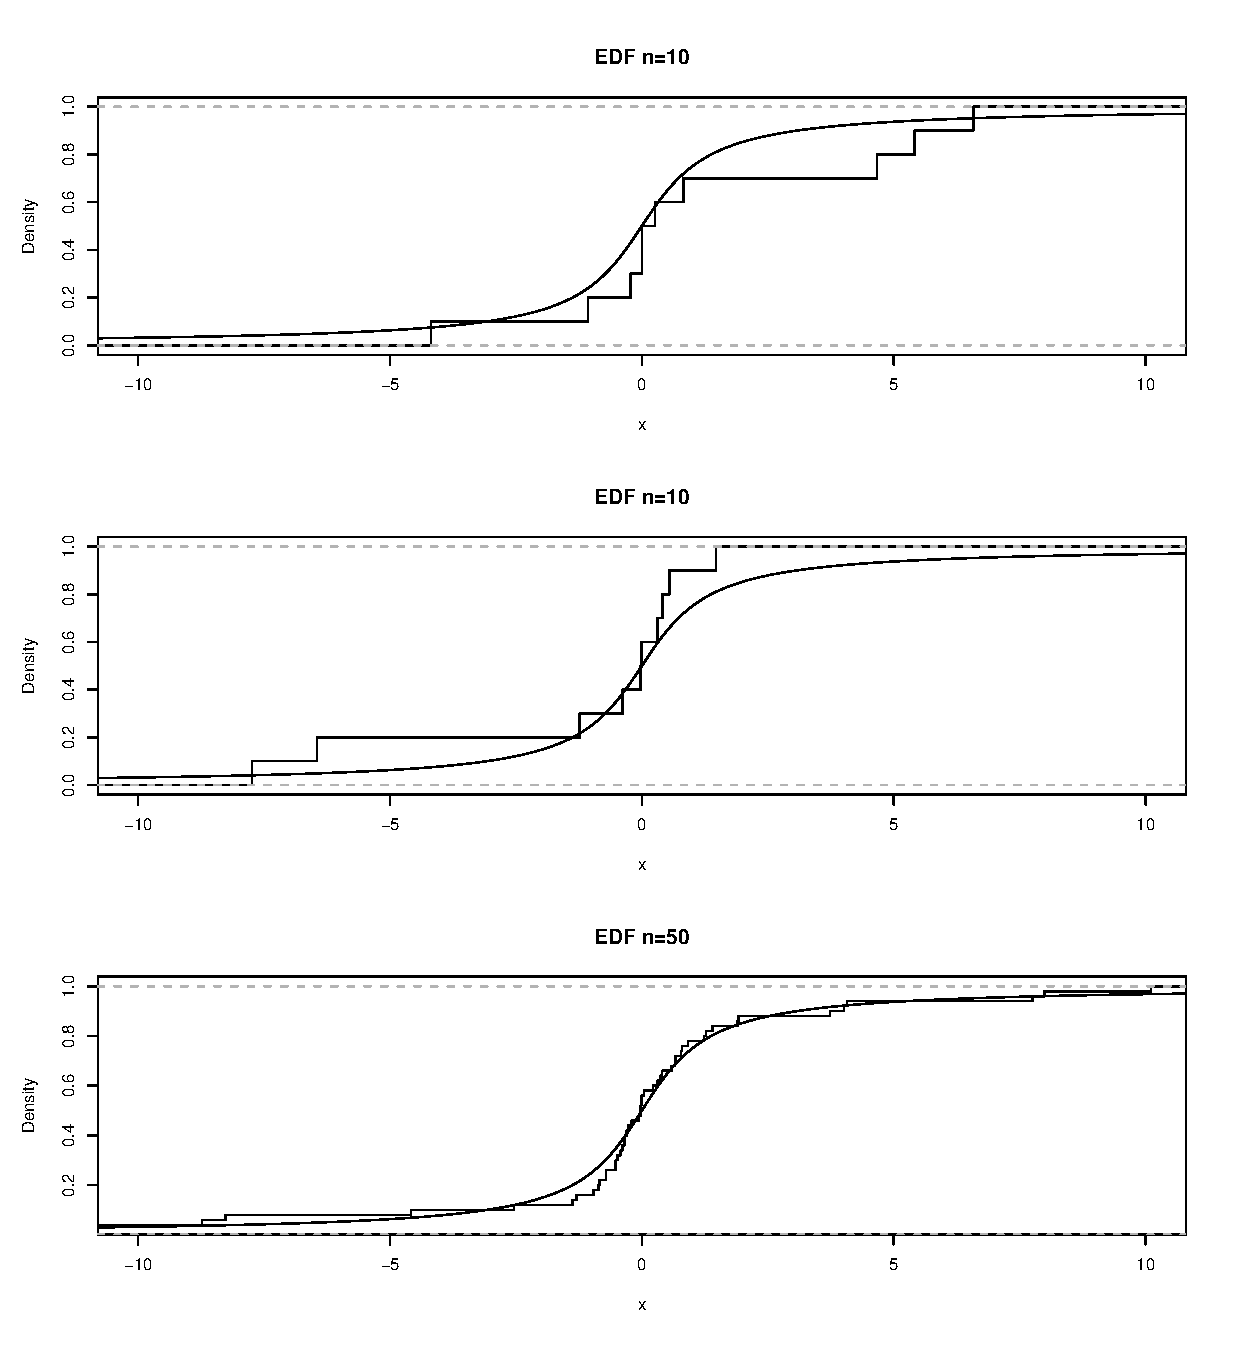
\includegraphics[scale=0.5]{CauchyEDF1.eps}
\end{center}
}

\frame{\frametitle{Example of the EDF - II}
\vspace{-1cm}
\begin{center}
 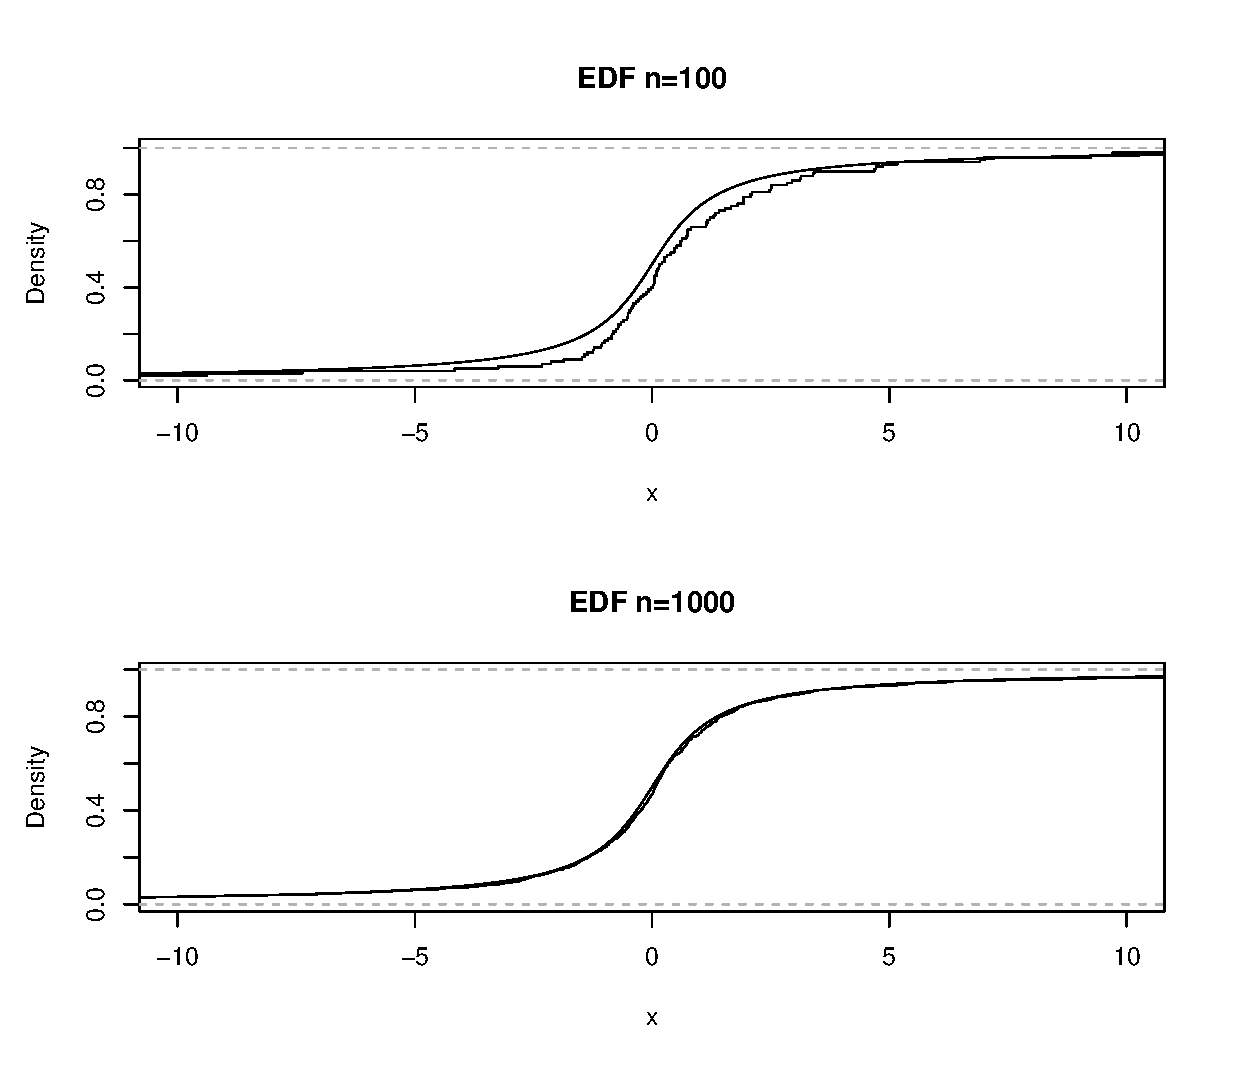
\includegraphics[scale=0.4]{CauchyEDF2.eps}
\end{center}

Notice that we've repeated for $n=10$ and that the edf is different each time. Notice also that the edf becomes more accurate as $n$ gets larger.
}



\frame{\frametitle{Parameters, statistics and properties}

Bootstrapping texts can sometimes be confusing because of the language usage. We say 
\begin{itemize}
 \item 
$\theta$ is a parameter if it is a property of the underlying population, i.e., $\theta=\theta(F)$. 

\item
 $\hat{\theta}$ is a statistic which estimates $\theta$ if $\hat{\theta}$ is a function of the sample $X_1, \ldots, X_n$ - this is equivalent to being a function of the empirical distribution function 
$$\hat{\theta}=\theta(\hat{F})\equiv \theta({X})$$
\item 
We then talk about properties  of $\hat{\theta}$ such as its bias, its expectation, its standard error  etc.  For bootstrapping applications these properties are usually sampling properties, that is, if we repeatedly collected similar samples, what properties would $\htheta$ have? 

\end{itemize}

Difficulties arise when we note that properties are also parameters of the statistic $\hat{\theta}$ and that we estimate them with statistics of the statistics.

}


\frame{\frametitle{Plug-in Principle}

For example, suppose we have a sample of size $n$, $\{X_1, \ldots, X_n\}$ say, from unknown density $F$. 

\medskip
Suppose that interest lies in some parameter $\theta$ of the distribution $F$ which we write $\theta=\theta(F)$ where we consider $\theta$ to be a functional  of the distribution $F$. 

\medskip
We estimate $\theta$ by $\hat{\theta}$ where $\htheta$ is a  function of the observations $\{X_1, \ldots, X_n\}$. Usually we have that $\htheta=\theta(\hF)$, that is, if we apply the functional $\theta(\cdot)$ to the edf $\hF$ we get the statistic $\htheta$.

\medskip
The parameter $\theta$ and the statistic $\htheta$ are both found by using the functional $\theta(\cdot)$. For the parameter we have $\theta=\theta(F)$, and for the statistic we have $\htheta=\theta(\hF)$. 

\medskip
This is what we call the {\it plug-in principle}. To estimate parameter $\theta=\theta(F)$ when we don't know $F$, we plug-in the empirical distribution function $\hF$ to find the estimator $\htheta=\theta(\hF)$.
 }
% 
% \frame{
% 
% How good is the plug-in principle? 
% 
% \medskip
% It is actually quite good if the only available information about $F$ comes from the sample $x$. Under these circumstances, $\htheta=\theta(\hF)$ is `optimal' in the traditional sense.
% 
% \medskip
%  For example, if $X_i \sim Bin(n, p_k)$ for $i=1, \ldots, N$ and if
% $\hat{p}_k$ is the plug-in frequency estimate ($\hat{p}_k=\frac{1}{N} \sum \BI_{X_i=k}$), then 
% $$\hat{p}_k\sim Bin(N, p_k)/N$$
% In this case, the estimator $\hat{p}_k$ is {\it unbiased} for $p_k$ and has variance $p_k(1-p_k)/N$. This is the smallest possible variance for any unbiased estimator of $p_k$.
% }
% 

\frame{\frametitle{Examples of parameters and the plug-in principle}
\begin{enumerate}
\item[1] {\bf Population mean} 
$$\theta=\theta(F)=\BE_F X=\int x \rm{d} F(x)=\int xf(x) \rm{d}x$$
Use the plug-in principle
{\color{blank}\begin{align*}
\htheta=\theta(\hF)&=\frac{1}{n}\int x\sum \mathbb{I}_{X_i \leq x}(\rm{d}x)\\
&= \frac{1}{n} \sum \int x \delta(x-X_i) \rm{d} x\\
&=\frac{1}{n} \sum X_i
\end{align*}
which is the sample mean, which is the usual estimator of the population mean.}
\end{enumerate}

}
\frame{
Here $\delta(x)$ is the Dirac delta function which is defined by its behaviour under integration 
$$\int_A \delta(x-a) \rm{d}x=\begin{cases} 1 \mbox{ if } a \in A\\
0 \mbox{ if } a \not \in A
\end{cases}
$$
The delta function $\delta(x-a)$ is the derivative of the indicator function $\BI_{x\leq a}$.
}

\frame{\frametitle{Examples of parameters and the plug-in principle}
\begin{enumerate}
\item[2] {\bf Population variance}
$$\theta=\theta(F)=\Var_F(X)=\int (x-\BE_F(X))^2 \rm{d} F(x)$$


{\color{blank}Using the plug-in principle we find that the statistic  $\htheta$ is 
\begin{align*}
 \htheta=\theta(\hF)&=\frac{1}{n}\int (x-\bar{X})^2\sum \mathbb{I}_{X_i \leq x}(\rm{d}x)\\
&=\frac{1}{n} \sum \int  (x-\bar{X})^2\delta(x-X_i) \rm{d} x\\
&=\frac{1}{n} \sum (X_i-\bar{X})^2
\end{align*}
This is not quite the usual estimator of variance ($\frac{1}{n-1} \sum (X_i-\bar{X})^2$) as usually we multiply this value by $n/(n-1)$ to get an unbiased estimator. $\htheta$ is biased in this case.}
\end{enumerate}
}



\frame{\frametitle{Examples of parameters and the plug-in principle}
\begin{enumerate}

\item[3] Probability $$\theta=\BP_F (X>c)=\int_c^{\infty} \rm{d} F(x)$$

{\color{blank}which is estimated by the statistic
$$\hat{\theta}=\frac{1}{n} \sum \mathbb{I}_{X_i>c}$$}

% \item[4] Median $$\theta=m \;\;s.t. \int_m^\infty \rm{d} F(x)=\frac{1}{2}$$
% estimated by the statistic
% 
% \begin{equation*}
% \hat{\theta}=\begin{cases} X_{(\frac{n+1}{2})} \mbox{ if } $n$ \mbox{ is odd}\\
% \frac{X_{(\frac{n}{2})}+X_{(\frac{n}{2}+1)}}{2} \mbox{ if } $n$ \mbox{ is even}\\
% \end{cases}
% \end{equation*}
% where $X_{(i)}$ are the order statistics of $\{X_1, \ldots, X_n\}$ 
\end{enumerate}
}


\frame{\frametitle{Sampling properties}
For our estimates to be of any value, it is necessary to know their properties, such as the bias or the standard error:
\begin{itemize}
\item
The bias is defined as 
$$\bias (\hat{\theta})=\BE \htheta-\theta$$

\item
The standard error is 
$$\se(\theta)=\sqrt{[ \BE (\htheta-\theta)^2]}$$

\end{itemize}
}


\frame{
If we believed that $X_i$ were from a specific parametric model $$\mbox{e.g. } F=\Phi \mbox{ so that } X_i \sim N(\mu, \sigma^2)$$
 then we could calculate the bias and standard error analytically. If these calculations were difficult or impossible (for example, if $\theta=$ trimmed mean) then we can use simulations from $F$ to estimate the standard error and bias of the statistics.


\medskip
What if we don't have a parametric model for $F$?

\medskip
 The bootstrap can be used to estimate the sampling distribution in this case.

\medskip
 The idea is that instead of sampling from the population of interest, i.e. from $F(\cdot)$, we instead sample with replacement from the sample $\{x_1, \ldots, x_n\}$, i.e. from $\hat{F}(\cdot)$. 
}



\frame{\frametitle{Heart-attack study}

A controlled, randomized, double-blind study was carried out to investigate whether or not aspirin reduces the risk of heart attacks in healthy middle-aged men. Data from the study is

\medskip
\begin{center}
\begin{tabular}{l|cc}
& heart attacks & subjects\\
&(fatal plus non-fatal)&\\
\hline
aspirin& 104 &11037\\
placebo & 189 &11034\\
\end{tabular}
\end{center}
}

\frame{\frametitle{Heart-attack study -II}

Define $\theta$ to be the true ratio of proportions of heart attacks in those with aspirin to those with a placebo, the relative risk. 

\medskip
From the data, the estimate of $\theta$ suggests that aspirin lowers the risk of a heart attack:
$$\htheta=\frac{104/11037}{189/11034}=0.55$$
But how confident can we be? 

\medskip
Can we calculate a confidence interval for $\theta$? 

\medskip
It is possible to derive a parametric  confidence interval for $\theta$ from theory by assuming that the log relative risk is normally distributed. But what if we've forgotten how, or don't wish to assume normality?

}

\frame{\frametitle{Heart-attack study -III}
Bootstrapping enables us to derive these intervals without assuming that the log relative risks are normally distributed:
\begin{enumerate}
\item Estimate the probability $\hat{p}_1$ of a patient with aspirin having a heart-attack:
$$
\hat{p}_1=\frac{104}{11037}=0.00942
$$
\item 
 Estimate the probability $\hat{p}_2$ of a patient with a placebo having a heart-attack:
$$
\hat{p}_2=\frac{189}{11034}=0.0171
$$

\item
Simulate data for a new experiment: sample $r_1$ from Binomial$(11037, 0.00942)$ and $r_2$ from Binomial$(11034, 0.0171)$. The new data is known as a bootstrap sample.

\item Obtain a new estimate of the ratio:
$$\htheta_s^*=\frac{r_1/11037}{r_2/11034}$$

\end{enumerate}
}

\frame{\frametitle{Heart-attack study -IV}
Steps 3 and 4 are then repeated a large number of times, to obtain a sample $$\{\htheta_1^*, \ldots, \htheta_B\}$$ 

We can then use the 2.5th and 97.5th percentiles of this sample as a 95\% confidence interval for $\theta$. 

\medskip
With $B=10000$, performing this procedure in R gave a 95\% interval of $(0.43, 0.69)$ for $\theta$.


\medskip

We will now formally introduce the bootstrap and look at some examples in detail.

}



\frame{\frametitle{The bootstrap}



The basic idea behind the bootstrap is to find properties of statistics $\htheta$ by resampling from $\hat{F}$ (rather than $F$). 
\begin{itemize}
 \item 

If we could generate from $F$, we could simulate sample data sets $\{X_1^{(i)}, \ldots, X_n^{(i)}\}$ for $i=1, \ldots, B$ and find $\htheta^{(i)}$. We can then learn properties of $\htheta$ from $\{\htheta^{(1)}, \ldots, \htheta^{(B)}\}$. 
\item
But usually we don't know $F$ and so can't produce these samples.

\item
 Instead we can use the bootstrap and replace $F$ by $\hF$.

\item
 We sample  from $\hF$ and find the properties of $\htheta$ under $\hF$.
\end{itemize}
}


\frame{\frametitle{The bootstrap}

\fbox{
\parbox{11cm}{\begin{enumerate}
 \item[]{\bf  The bootstrap algorithm}
 \item Generate $B$ bootstrap replicates from $\hat{F}$.
 $${\bf X}^{*(i)}=\{X_1^{*(i)}, \ldots, X_n^{*(i)}\} \mbox{ for } i=1, \ldots, B$$

 \item Calculate $B$ bootstrap parameter estimates
 $$\htheta_1^*, \ldots, \htheta_B^*$$
 
 \item Calculate the property of interest for $\htheta$ from $\{\htheta_i^*\}_{i=1}^B$
 e.g. 
 $$\se_{boot}(\htheta)=\sqrt{\BE_F(\htheta-\theta)^2}\approx\sqrt{\frac{1}{B-1}\sum (\htheta_i^*-\bar{\htheta})^2}$$
 where $\bar{\htheta}=\frac{1}{B}\sum \htheta_i^*$
 
 \end{enumerate}}}
}


\frame{\frametitle{The bootstrap}

We call iid samples of size $n$ from $\hat{F}$ {\it bootstrap replicates}. 

\medskip
They can be generated by sampling with replacement from $\{x_1, \ldots, x_n\}$. 

\medskip
In R this can be achieved by using the command\\

\texttt{ sample(n=1, size=n, data=x, replace=T)}

}






\frame{\frametitle{The bootstrap estimate of standard error}

Suppose $\htheta(X)$ is some statistic based on $X=\{x_1, \ldots, x_n\}$ used for estimating parameter $\theta$.
The standard error of $\htheta(X)$, denoted as $\se(\htheta)$ is 
$$\se(\htheta)=\sqrt{\Var_F(\htheta(X))}$$


Here the variance is with respect to distribution $F$.


\medskip
The bootstrap estimate is found by replacing $F$ with $\hF$.
$$\se_F(\hat{\theta}) \stackrel{\scriptsize{O_p(\frac{1}{\sqrt{n}})}}{\approx} se_{\hat{F}}(\hat{\theta}) \stackrel{O_p(\frac{1}{\sqrt{B}})}{\approx} \left( \frac{1}{B-1} \sum_{b=1}^B (\hat{\theta}(X^{(b)}) - \bar{\hat{\theta}})^2 \right) ^{\frac{1}{2}} =: \se_{boot}$$
where $X^*=\{X_1^*, \ldots, X_n^*\}$ is a bootstrap sample from $\{x_1, \ldots, x_n\}$,  ie, $\se_{boot}^2$ is the variance of $\htheta(X^*)$ when $X^*$ are drawn from $\hF$. 


Here $Y_n = O_p(x_n)$ means that $Y_x/x_n$ is stochastically bounded, i.e., for any $\epsilon>0$, there exists $M>0$, such that for all $n$
$$\BP(|Y_n/x_n| > M) <\epsilon$$

}

\frame{\frametitle{The bootstrap estimate of standard error - II}

This is the plug-in principle again. If we consider the variance of $\htheta$ to be a functional of $F$ - 
$$\Var(\htheta)[F]=\BE_F(\htheta- \BE_F(\htheta))^2$$
then when we plug-in $\hF$ we find

$$\Var_{\hat{F}}(\htheta)=\BE_\hF(\htheta-\BE_\hF\htheta)^2.$$
}


\frame{\frametitle{The bootstrap estimate of standard error - III}

We can estimate $\se_{boot}$ empirically by replacing $\Var_\hF(\htheta(X^*))$ with an estimate
$$\Var_\hF(\htheta(X^*))\approx \Var_{boot}(\htheta(X^*))= \frac{1}{B-1} \sum_{b=1}^B (\htheta(X^{*(b)})-\bar{\htheta})^2$$
where 
$$\bar{\htheta}=\frac{1}{B}\sum_{b=1}^B \htheta(X^{*(b)})$$
and where
$$X^{*(b)}=\{X^{*(b)}_1, \ldots, X_n^{*(b)}\}$$ are $B$ bootstrap replicates from $\hF$.

}



\frame{\frametitle{Bootstrap estimate of bias}
The bias of an estimator $\htheta$ of parameter $\theta$ is defined as
$$\bias=\BE_F(\htheta)-\theta$$
i.e., how the mean of the estimator of $\theta$ differs from the true value of $\theta$. 

\medskip
An estimate is found by replacing $F$ by $\hF$.
$$\bias_{\hF}=\BE_\hF(\htheta)-\htheta$$
That is, the difference between the expected value  and the estimated value. 

}

\frame{\frametitle{Bootstrap estimate of bias - II}
Clearly, for large $B$, we can estimate $\BE_\hF(\htheta)$ from bootstrap samples as
$$ \BE_\hF(\theta)\approx \frac{1}{B} \sum_{b=1}^B \htheta^*_{(b)}$$

This is again the plug-in principle. If we consider bias to be the functional $\bias(F)=\BE_F(\htheta)-\theta(F)$ then when we plug-in $\hF$ we find
\begin{align*}
\bias_{\hF}(\htheta)&=\BE_\hF(\htheta)-\theta(\hF)=\BE_\hF(\htheta)-\htheta\\
&\approx \bias_{boot}(\htheta) = \frac{1}{B} \sum_{b=1}^B \htheta^*_{(b)} - \htheta
\end{align*}


}


\frame{
So in general there are two aspects to the bootstrap procedure:
\begin{enumerate}
 \item Replace $F$ by $\hF$.
\item Simulate from $\hF$ to form the estimate of the property of interest.
\end{enumerate}

}

% 
% 
% \frame{\frametitle{Theoretical calculation}
% 
% For certain statistics and certain properties we can calculate the bootstrap exactly.
% 
% \medskip
%  For example, suppose the parameter of interest is $\theta=\BE_F(X)$ so that the statistic is $\htheta(X)=\bar{X}$, and that we wish to calculate its standard error (the property). 
% 
% \medskip
% Then in this case we can calculate the bootstrap estimate without resorting to simulation 
% 
% }
% 
% 
% \frame{\frametitle{Empirical calculation}
% In some simple cases it is possible to analytically calculate. However, usually we must revert to Monte Carlo methods.
% 
% \medskip
%  So for the example with the standard error of the mean,
% the Monte Carlo estimate would be to generate $B$ bootstrap replicates $$\{x^{*(j)}_1, \ldots, x_n^{*(j)}\}$$ and for each set calculate the sample mean $\bar{x}^{(j)}$.
% 
% \medskip
%  Repeat this $B$ times and then calculate the variance of these bootstrap replicates
% $$\Var_\hF(\htheta(X^*))\approx \frac{1}{B-1} \sum_{b=1}^B (\bar{x}^{*(b)}-\bar{\bar{x}})^2$$
% where $\bar{\bar{x}}=\frac{1}{B} \sum_{b=1}^B \bar{x}^{*(b)}$.
% 
% }
% 


\frame{\frametitle{Lawschool example}

A sample of 15 law schools was taken, and two measurements were made for each school:
\begin{center}
\begin{tabular}{ll}
 $x_i:$  &LSAT, average score for the class on a national law test\\
$y_i:$ &GPA, average undergraduate grade-point average for the class\\
\end{tabular}
\end{center}
We are interested in the correlation coefficient between these two quantities, which we estimate to be $\htheta=0.776$.

\vspace{-0.7cm}
\begin{center}
 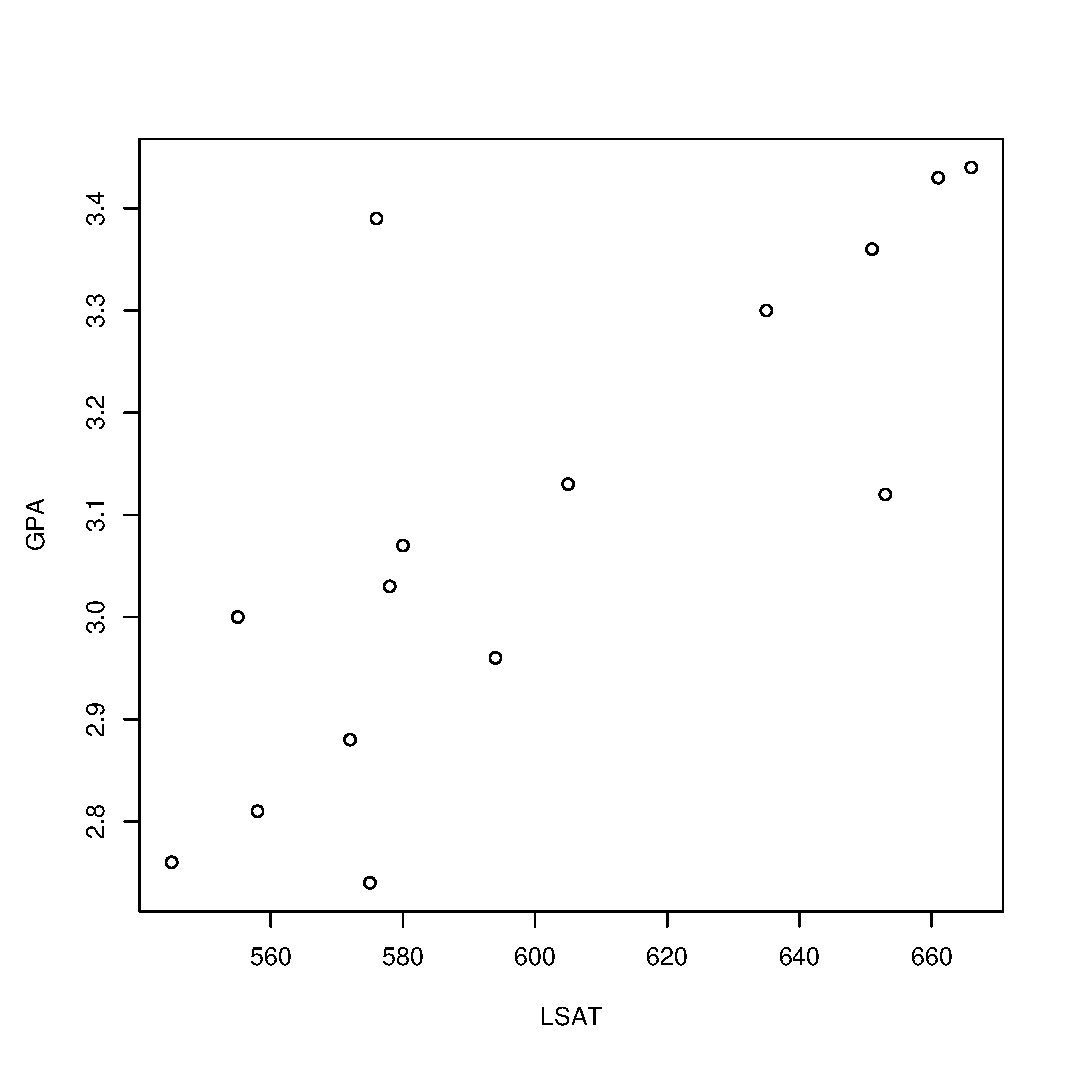
\includegraphics[scale=0.3]{Law.eps}
\end{center}
}

\frame{\frametitle{Lawschool example - II}
But how accurate is this estimate of the correlation coefficient? We use the  bootstrap to estimate the standard error of $\htheta=\cor(LSAT, GPA)$.

\begin{enumerate}
 \item Sample 15 data points with replacement from the observed data $z=\{(x_1, y_1), \ldots, (x_{15}, y_{15})\}$ to obtain new data $z^*$.
\item Evaluate the sample correlation coefficient $\htheta^*$ for the newly sampled data $z^*$.

\item Repeate steps 1 and 2 to obtain $\htheta^{*(1)}, \ldots, \htheta^{*(B)}$.
\item Estimate the standard error of the sample correlation coefficient by the sample standard deviation of $\htheta^{*(1)}, \ldots, \htheta^{*(B)}$.

\end{enumerate}
}

\frame{\frametitle{Lawschool example - III}
With $B=1000$, I found the estimated standard error of $\htheta$ is 0.137. It can help to plot a histogram of the bootstrap replicates as this gives more information about the distribution of $\htheta$.

\begin{center}
%\psfrag{Theta}[][][][]{$\htheta$}
 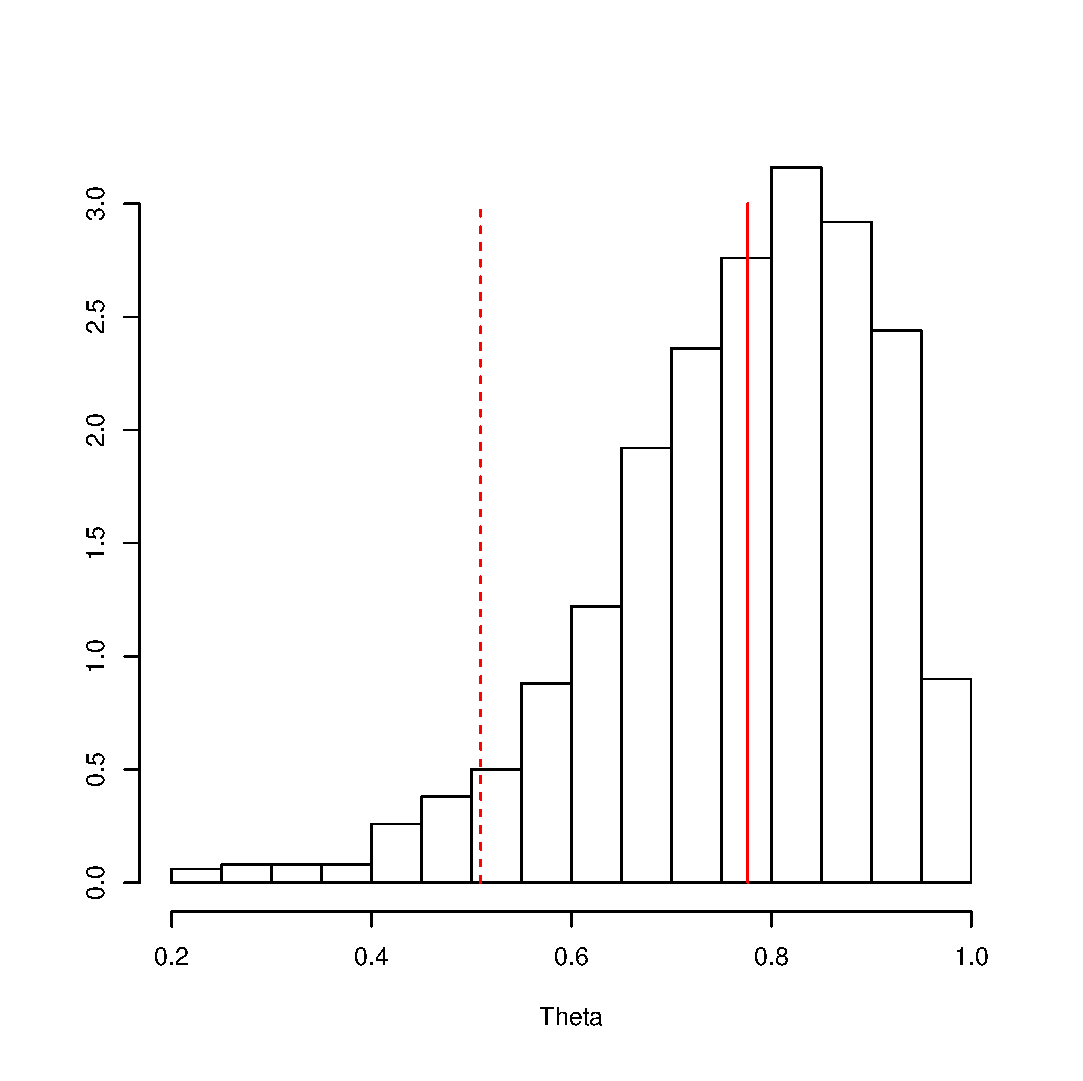
\includegraphics[scale=0.35]{LawBootReplicates.eps}
\end{center}
}

\frame{\frametitle{Bootstrap confidence interval}
We have two methods of calculating CIs.
\begin{itemize}
\item[1] Given an estimate of the standard error of $\htheta$, if we assume that the distribution of $\htheta$ is approximately normal, then an approximate 95\% confidence interval is given by 
$$\htheta\pm 1.96\se(\htheta^*)$$
\begin{itemize}
\item For the law dataset we find a 95\% CI for $\cor(LSAT, GPA)$ of $[0.51, 1.04]\equiv[0.51, 1.00]$.
\end{itemize}
\end{itemize}

}

\frame{\frametitle{Bootstrap confidence interval - II}
\begin{itemize}
\item[2] {\bf Percentile confidence interval}

For a 95\% confidence interval, we need to find the two values $l$ and $u$ with 
\begin{align*}
 \BP(\htheta^*>u)&=0.975\\
\BP(\htheta^*<l)&=0.025
\end{align*}
ie, we need to identify 2.5th and 97.5th percentiles from the distribution of $\htheta^*$. We can find this from the 2.5th and 97.5th percentiles of the sample $\{\htheta^{*(1)}, \ldots, \htheta^{*(B)}\}$. We generally need a larger value of $B$ to get accurate percentile estimates than that required to find an accurate estimate of the standard error.
\begin{itemize}
\item For the law dataset we find a 95\% CI of $[0.45, 0.96]$.
\end{itemize}
\end{itemize}
%R code for these calculations is available in \texttt{LawExample.txt}.
}


%\frame{\frametitle{The Jackknife}
%
%The jackknife predates the bootstrap, and is a less general method. However, it is still used and so we will study it. Let $x_{(i)}$ be the data set with the $i^{th}$ datum removed so that
%$$x_{(i)}=(x_1, x_2, \ldots, x_{i-1}, x_{i+1}, \ldots, x_{n}),$$ and let $\htheta_{(i)}$ be the statistic $\htheta$ evalutated for the data set $x_{(i)}$. Then the jackknife estimate of the standard error of $\htheta$ is given by
%$$
%\se_{jack}(\htheta)=\left(\frac{n-1}{n}\sum_{i=1}^n (\htheta_{(i)}-\bar{\htheta}_{(\cdot)})^2 \right)^{1/2}$$
%where
%$$\bar{\htheta}_{(\cdot)}=\frac{1}{n}\sum_{i=1}^n \htheta_{(i)}$$
%}
%
%
%\frame{
%If $\htheta=\bar{x}$ then it can be shown that
%$$\htheta_{(i)}=\frac{1}{n-1} \sum_{j\not=i} x_j \mbox{ and  } \bar{\htheta}_{(\cdot)}=\bar{x}$$
%Hence the jackknife estimate of standard error in this case reduces to
%
%$$\se_{jack}(\htheta)=\sqrt{\frac{\sum(x_i-\bar{x})^2}{n(n-1)}}$$
%which is the usual unbiased estimate of the standard error.
%
%For the law example we find the jackknife estimate of standard error is $0.1425$.
%}
%
%\frame{\frametitle{Jackknife estimate of bias}
%The Jackknife estimate of bias is
%
%$$\bias_{jack}(\htheta)=(n-1) (\BE_\hF (\htheta)-\htheta).$$
%ie, it  is the difference between  the expected value of the empirical distribution and the estimated value, so this is simply
%
%$$(n-1)(\bar{\htheta}_{(\cdot)}-\htheta).$$
%
%If $\htheta=\bar{x}$ then we can show that the estimate of bias is zero, i.e., we have an unbiased estimator. 
%
%For the law example, we find the bias of $\htheta$ is $-0.0065.$
%}
%
%


\frame{\frametitle{Hypothesis testing with the
bootstrap}\pause

\textbf{Example: mice survival times}
\begin{center}
\begin{tabular}{c|ccccccccc}
Treatment& 94& 197& 16& 38&99&141&23& & \\ \hline Control &
52&104&146&10&50&31&40&27&46
\end{tabular}
\end{center}\pause

Is there a difference between two group means?\pause


\begin{itemize}
\item Denote 7 treatment observations by ${\bf x}=\{x_1,\ldots,x_7\}$,
and 9 control observations by ${\bf y}=\{y_1,\ldots,y_9\}$.\pause \item
Could perform two-sample $t$ test, assuming normally distributed
responses and equal variances in the two groups.\pause \item Define
$\mu_X$: population treatment mean, $\mu_Y$: population control
mean. For one-sided test of $H_0:\mu_X=\mu_Y$, observed $p-$value is
0.1405.

\end{itemize}}

\frame{

\begin{block}{Bootstrap hypothesis test}\pause

\begin{itemize}
\item Alternative to assuming normality\pause
\item Denote $F_X$: distribution of treatment survival time, $F_Y$:
distribution of control survival time.\pause \item Write null
hypothesis as $H_0:F_X=F_Y=F$, with $F$ the single common
distribution of all the responses. \pause\item estimate $F$ by
$\hat{F}$, empirical cdf of all 16 observations.
\end{itemize} \end{block}
}

\frame{

Bootstrap two-sample significance test\pause

\begin{enumerate} \item
 Sample 16 values with
replacement from $\{x_1,\ldots,x_7,y_1,\ldots,y_9\}$. \pause \item
Set $\{x_1^*,\ldots,x_7^*\}$ to be the first 7 sampled values, and
$\{y_1^*,\ldots,y_9^*\}$ to be the remaining 9 sampled values.
\pause \item Calculate the bootstrap test statistic
$$T^*=\frac{\bar{x}^*-\bar{y}^*}{\hat{\sigma^*}\sqrt{1/7+1/9}}$$
for the sampled data.\pause \item Repeat steps 1 to 3 $B$ times to
obtain $T^*_{(1)},\ldots,T^*_{(B)}$. \pause \item Estimate the
significance of the observed $T_{obs}$ by
\begin{equation}
\frac{1}{N}\sum_{i=1}^N I\{T^*_{(i)}\ge T_{obs}\}
\end{equation}

\end{enumerate}

}

% 
% 
% \frame{\frametitle{One sample hypothesis tests}\pause Mice
% example: from previous studies believe that $\mu_X=100$. Could test
% this with one sample $t$ test.\pause
% 
% Two-sided $t$-test of $H_0:\mu_X=100 $ gives $p-$value 0.6212 for
% $T_{obs}=\frac{86.9-100}{\hat{\sigma}/\sqrt{7}}, $ with
% $\hat{\sigma}$ the sample standard deviation, equal to 66.8.\pause
% 
% One sample bootstrap test. \pause \begin{itemize}\item Always
% approximate distribution $F$ by empirical cdf. \pause \item But from
% empirical cdf, expectation of single observation is sample mean
% 86.9, not 100 as stated by $H_0$. \pause \item Need to transform
% data:
% \begin{equation}
% x_i'=x_i-86.9+100.
% \end{equation}\pause
% \item Assumption is that distribution $F$ will have same
% \textit{shape} for any value of the true mean $\mu_X$. (may need log
% transformation if must have $X>0$.\pause \item Use empirical cdf to
% estimate shape of $F$.
% 
% \end{itemize}
% 
% }
% 
% \frame{
% 
% \frametitle{Bootstrap one-sample significance test}\pause
% 
% \begin{enumerate}
% \item Transform the data such that the sample mean equals the mean
% under $H_0$: $x_i'=x_i-\bar{x}+\mu_X$\pause
% \item Sample 7 values with replacement from\\
% \{107.1,210.1,29.1,51.1,112.1,154.1,36.1\} to obtain new data
% ${\bx'}^*$ \pause \item Re-evaluate the test statistic for the new
% data:$$T^*=\frac{\bar{x'}^*-100}{\hat{\sigma}'^*/\sqrt{7}},$$ where
% $\hat{\sigma}'^*$ is the sample standard deviation of the new
% data\pause
% \item
% Repeat steps 2 and 3 $N$ times to obtain
% $T^*(1),\ldots,T^*(N)$.\pause
% \item Estimate the significance of $T_{obs}$ by
% $$\frac{1}{N}\sum_{i=1}^NI\{T^*(i)\ge T_{obs}\} $$
% 
% \end{enumerate}
% 
% }
% 


\frame{\frametitle{The Bootstrap and Regression}

A formal regression type model has the structure

$$y_i=f(x_i, \beta) +\epsilon_i$$
where $f$ is a specified function acting on the covariates $x_i$ with parameters $\beta$, and $\epsilon_i$ is a realisation from a specified error structure. With this model framework, there are two alternative ways to bootstrap the model.

\begin{enumerate}
 \item Fit the regression model, form the empirical distribution of the residuals, generate bootstrap replications of the data by substituting these back into the model, and re-fit the model to obtain bootstrap distributions of $\beta$. This is called {\it model-based resampling}.

\item Bootstrap from the pairs $(x_i, y_i)$, re-fit the model to each realization, form the bootstrap distribution of $\beta$. 

\end{enumerate}
}

\frame{\frametitle{Model-based resampling}

We will fit a model of the form
$$GPA_i=\beta_0+\beta_1 LSAT_i+\epsilon_i$$ to the law data. A least squares fit to these data gives $\hat{\beta}_0=0.3794$ and $\hat{\beta}_1=0.0045$, but how accurate are these values? We can perform the following set of steps to find the standard error of these estimates
}

\frame{\frametitle{Model-based resampling - II}

\fbox{
\vspace{-0.5cm}
\parbox{11cm}{
\begin{enumerate}
\item Find the fitted residuals
$$\hat{\epsilon}_i=GPA_i-\hat{\beta}_0-\hat{\beta}_1 LSAT_i$$

\item Sample $\epsilon^*_1, \ldots, \epsilon^*_{15}$ with replacement from $\{\hat{\epsilon}_1,\ldots,\hat{\epsilon}_{15}\}$

\item  $$\mbox{Set } GPA_i^*=\hat{\beta}_0+\hat{\beta}_1 LSAT_i+\epsilon^*_i$$

\item Fit the least squares regression to $\{(LSAT_1, GPA_1^*), \ldots, (LSAT_{15}, GPA_{15}^*)\}$ to find estimates $\beta=(\beta_0^*, \beta_1^*)$.

\item Repeat steps 2 to 4 $B$ times to find bootstrap replicates 
$$\{(\beta_0^{*(1)}, \beta_1^{*(1)}), \ldots,(\beta_0^{*(B)}, \beta_1^{*(B)})\}$$
and use these replicates to estimate $\se(\hat{\beta}_0)$ and $\se(\hat{\beta}_1)$.
\end{enumerate}
}}
}


\frame{\frametitle{Model-based resampling - III}
Using 1000 bootstrap replicates, I find the standard errors are
$$\se(\hat{\beta}_0)=0.586, \qquad \se(\hat{\beta}_1)=0.000973$$
and the plot shows a sample of 20 bootstrap regression lines.
\vspace{-0.5cm}
\begin{center}
 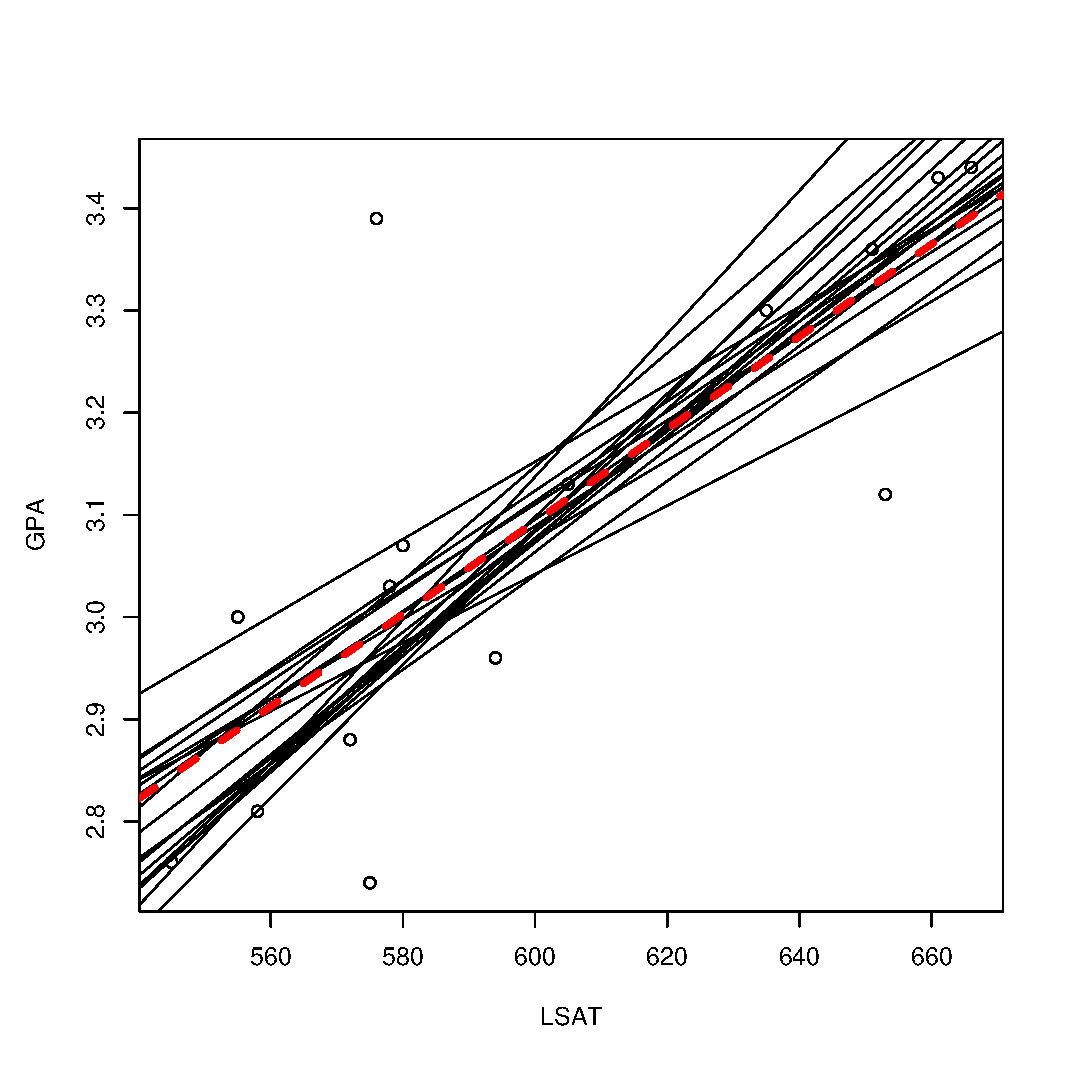
\includegraphics[scale=0.4]{LawRegression.eps}
\end{center}

}


\frame{\frametitle{Motorcycle example}

We consider data providing measurements of acceleration against time for a simulated motorcycle accident. The data are shown in the figure.

\vspace{-0.5cm}
\begin{center}
 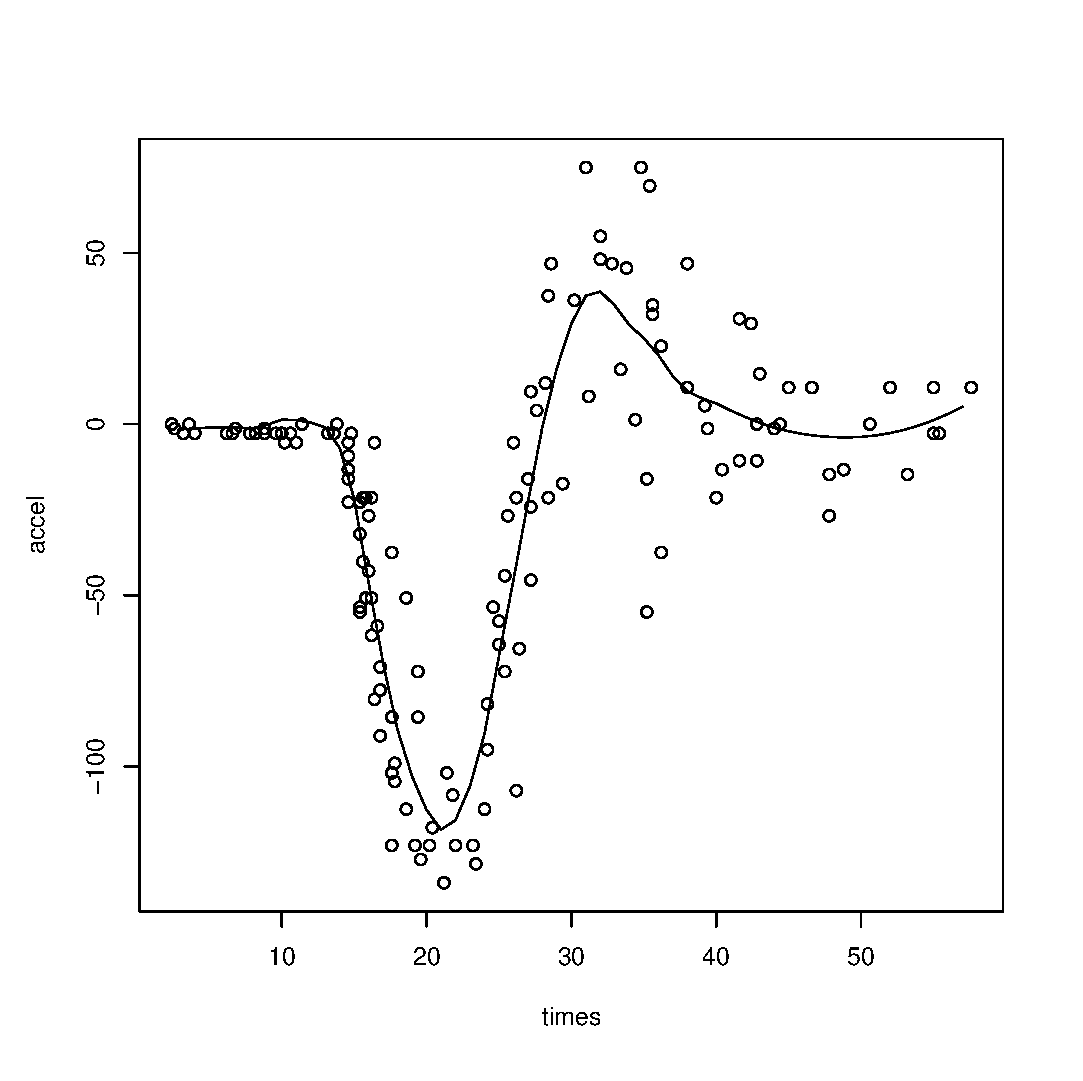
\includegraphics[scale=0.4]{Motorcycle.eps}
\end{center}
}

\frame{\frametitle{Motorcycle example}
Clearly the relationship is nonlinear, and has structure that will not easily be modelled parametrically. We use the {\texttt loess()} command in R to fit a locally weighted least-squares regression line to the data (the details aren't important for this course, but for completeness sake we set {\texttt span=1/3} which determines the proportion of the data to be included in the moving window which specifies which points are to be regressed upon.). The figure shows the best fit.  

Because of the non-parametric structure of the model, classical approaches to the assessment of parameter precision are not available. 
We can get a sense of how accurate the parameters are by using a bootstrapping scheme (of the first type). This is achieved by simply bootstrapping the pairs (x,y) in the original plot and fitting {\texttt loess} curves to each simulated bootstrap series. A figure showing 20 bootstrap samples is shown below.

}

\frame{\frametitle{Motorcycle example}
\vspace{-1cm}
\begin{center}
 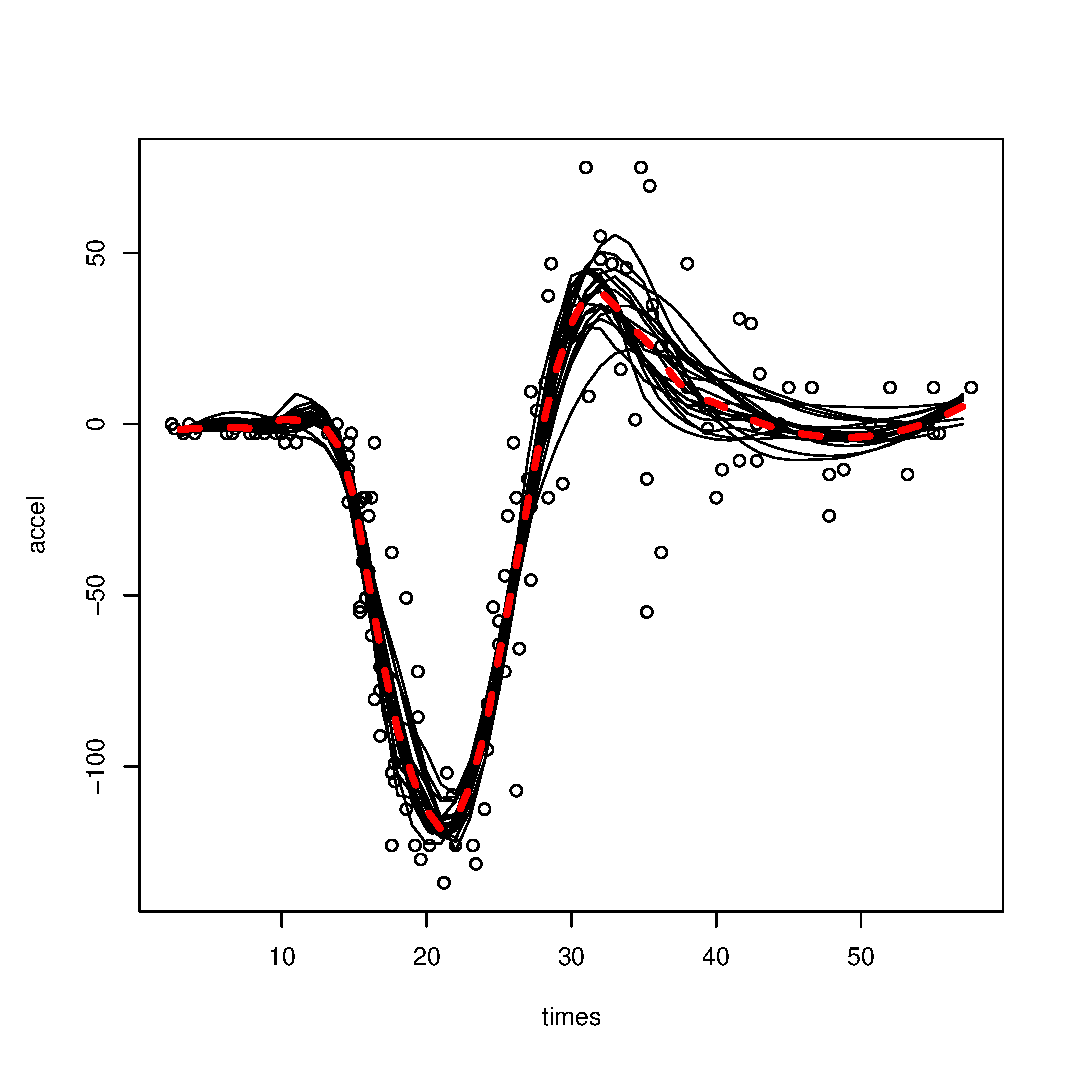
\includegraphics[scale=0.5]{MotorcycleBoot.eps}
\end{center}

R code is available in \texttt{motorcycle.txt}.

}



\frame{\frametitle{Summary}

\begin{enumerate}\item Monte Carlo tests\pause
\begin{itemize}
\item Will work with any test statistic and hypothesis, but
requires specification of distribution of data under null
hypothesis\pause
\item Only procedure out of three that
produces `completely new' data.
\end{itemize}\pause

\item Randomization tests
\begin{itemize}\pause
\item Can generally only handle tests of no treatment effect
between different treatment groups. One sample tests can be
performed, but under stricter assumptions.\pause \item No
distribution is required/assumed for the data, only that allocation
of subjects to treatment groups is random.\end{itemize}

\end{enumerate}

}

\frame{

\begin{enumerate}\item[3] Bootstrapping\pause
\begin{itemize}
\item  Arguably the most widely applicable method of the three.\pause
\item Main use is to construct confidence intervals\pause  \item
Dependent on the empirical cdf being a good approximation to the
true distribution.\pause \item Accuracy ultimately depends on size
of \textbf{original} sample.

\end{itemize}
\end{enumerate}

}



\frame{\frametitle{2.4 Prediction errors and cross-validation}

A useful computational tool for assessing the performance of a model (eg a regression or classification model) is in terms of its {\it predictive} ability. 
\medskip

In data-rich environments, we can simply split the data into a training set, and a test set. We fit the model on the training-set, and then test its predictive accuracy on the test set. 

\medskip

However, if we do not have a lot of data, then we can't `waste' some by leaving in a test set and not using it in training.

\medskip
Prediction can be assessed efficiently within the framework of bootstrapping, but here we will consider an alternative method known as {\it cross-validation}.
}

\frame{\frametitle{Cross-validation in regression}

Given data $\{(x_1, y_1), \ldots, (x_n, y_n)\}$, then we can always fit this data perfectly with a polynomial of degree $n-1$, so that the sum of the squared errors is 0.
\vspace{-0.5cm}
\begin{center}
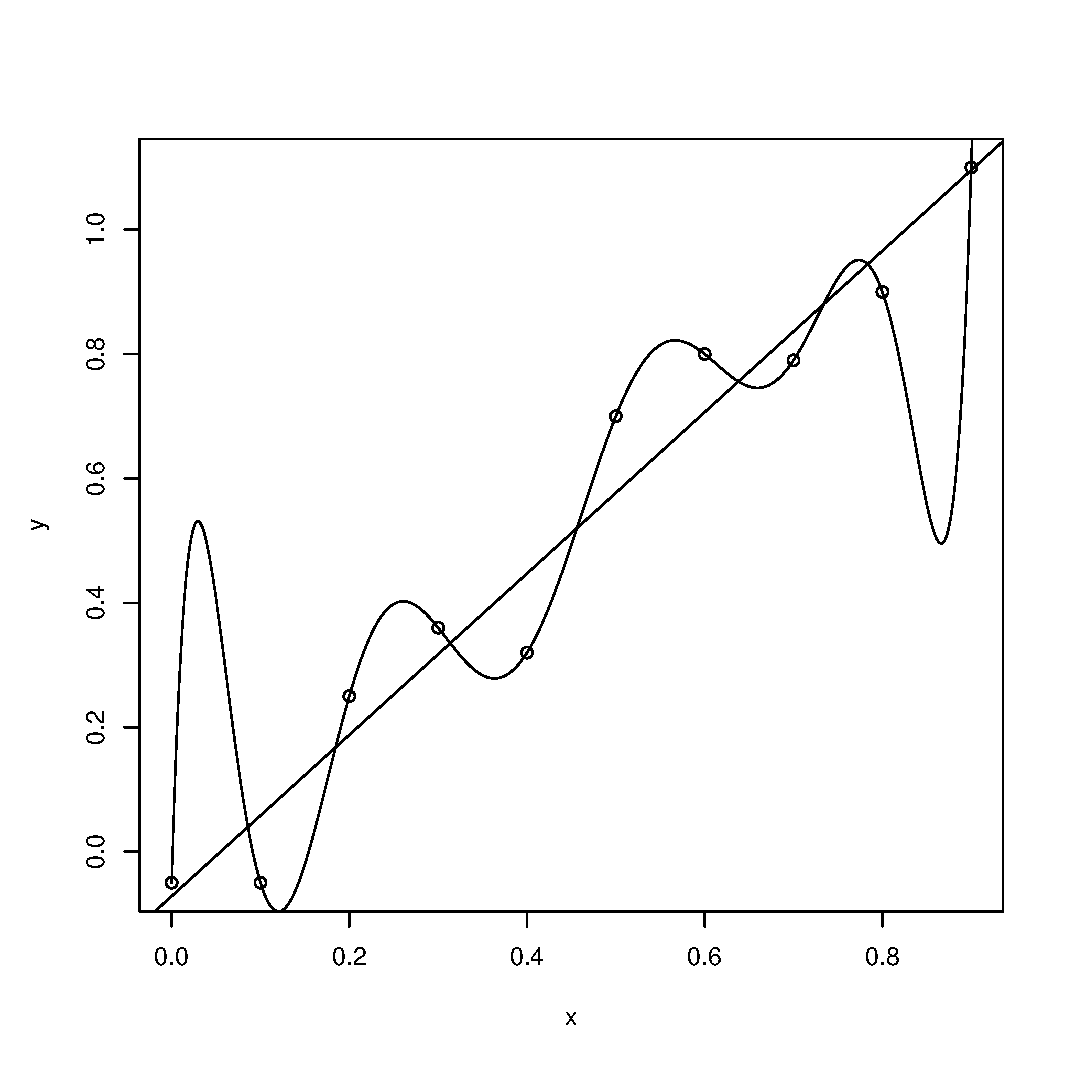
\includegraphics[scale=0.4]{polynomial.eps}
\end{center}
}


\frame{
\begin{quotation}
With four parameters I can fit an elephant, and with five I can make him wiggle his trunk. John von Neumann\end{quotation}

Of course, we know in general that fitting high order polynomials to regression data is not a sensible thing to do, but how can we demonstrate this? 

\medskip
With more data, we could check the predictions from this model against the new observations. However, its not always going to be possible to obtain new data just to check the performance of a model.

\medskip
The idea of cross-validation is to divide the data into two parts, a {\it training-set} to fit the model to, and a {\it test-set} to test the predictive performance. 

}

\frame{
\vspace{1cm}
\fbox{
\parbox{11cm}{ {\bf Leave-one-out cross-validation}
For $i=1, \ldots, n$
\begin{enumerate}
\item Fit the model to the reduced data set (or training set),
$$\{(x_1, y_1), \ldots, (x_{i-1}, y_{i-1}), (x_{i+1}, y_{i+1}), \ldots, (x_n, y_n)\}$$
\item Obtain from the fitted model the predicted value $\hat{y}_i$ at $x_i$.

\item Compute the squared error $\epsilon_i=(\hat{y}_i-y_i)^2$
\end{enumerate}
 An average squared prediction error can then be reported as $\frac{1}{n}\sum_{i=1}^n \epsilon_i^2$, or the root-mean-square (rms) prediction error as $\sqrt{\frac{1}{n}\sum_{i=1}^n \epsilon_i^2}$.
}}\\

}

\frame{
Note that this is not the expected prediction error of the actual model, though it should be close if $n$ is sufficiently large (so that the fit to $n-1$ points is very similar to the fit to $n$ points). 

\medskip
This approach left out one point at a time, and is called {\bf leave-one-out cross-validation}. 

\medskip
A variant is to remove subsets of size $k$ from the data each time, so that the training set has $n-k$ observations and the test set has $k$ observations. This is known as {\bf k-fold cross-validation}.


}


\frame{

\medskip
We remove a single point from the data set, and fit both models to the nine remaining observations. The left out value is predicted and compared to the actual value. 
\vspace{-0.5cm}
\begin{center}
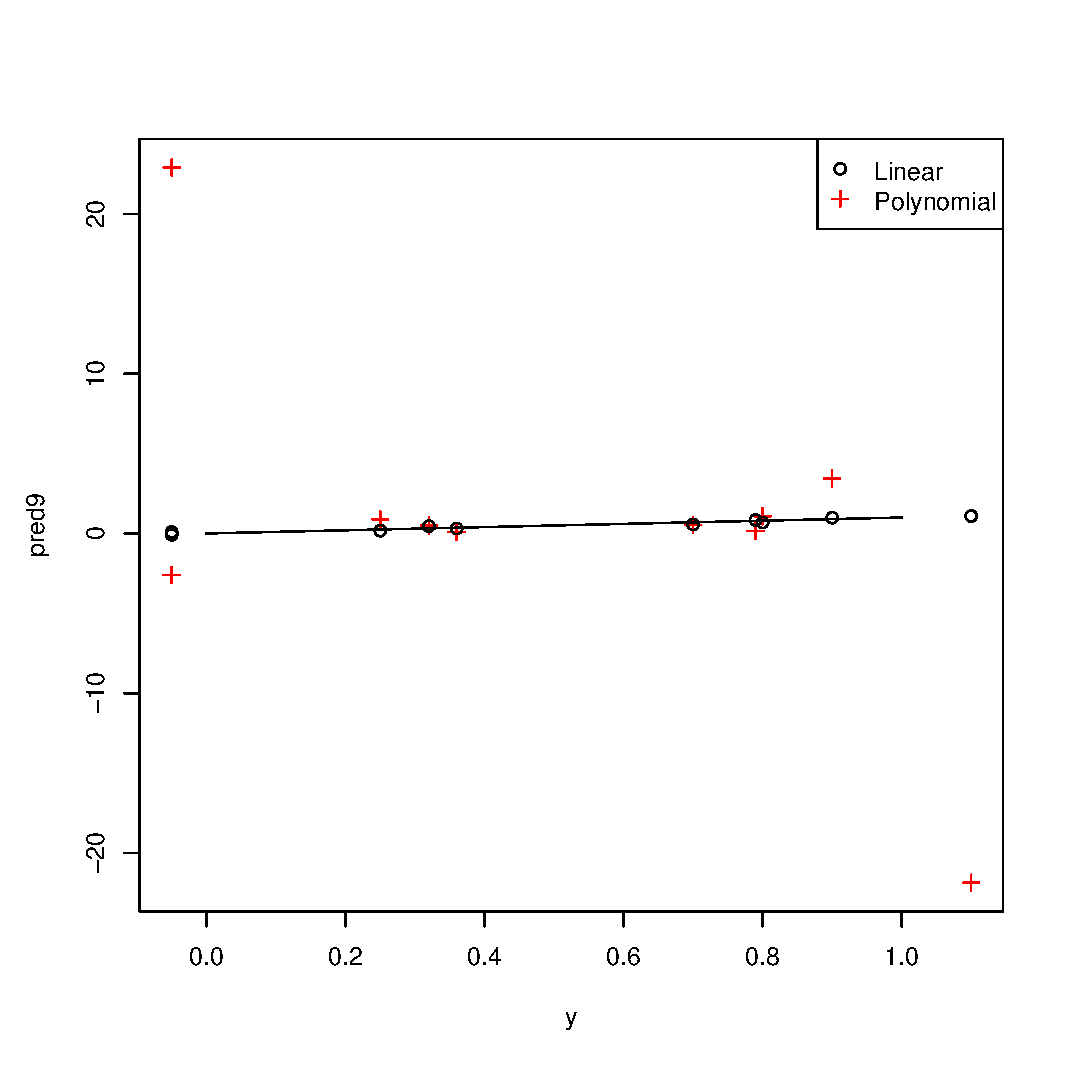
\includegraphics[scale=0.35]{CV.eps}
\end{center}

\vspace{-0.5cm}
We can see that linear regression is much better in terms of predictive performance. The rms prediction error for the straight line is 0.0955 whereas for the 8th order polynomial it is 10.34. 





}





\end{document}


